\documentclass[a4paper, 12pt]{article}

% Добавляем новые пакеты
\usepackage[english, russian]{babel}    % Пакет для поддержки русского языка
\usepackage[T1, T2A]{fontenc}           % Загружаем пакет с поддержкой кирилицы
\usepackage[utf8]{inputenc}             % Загружаем пакет с поддержкой кодировки файла и символов
\usepackage{ragged2e}                   % Загружаем пакет для выравнивания текста
\usepackage{graphicx}                   % Загружаем пакет для добавления различной графики (pdf, jpg, png)
\usepackage{import}                     % Загружаем пакет для продвинутого импорта, в частности изображений pdf_tex из графического редактора inkscape (\import{<path to file>}{<filename>.pdf_tex})
\usepackage{subcaption}                 % Пакет для поддержки сетки из фигур, например в две колонки или матрицей
\usepackage{float}                      % Пакет для улучшенного размещения изображенией (ниже используется опция H в команде \begin{figure}[H])
\usepackage{geometry}                   % Пакет для управления отступами на странице (см. далее вызываем \geometry)
\usepackage{amsmath}                    % Добавляем крутую поддержку математики, в частности /align
\usepackage{amsfonts}                   % Пкет с мтематическими шрифтами вроде \mathbb и др.
\usepackage{tabu}                       % Пакет с прокаченными таблицами
\usepackage{booktabs}                   % Крутые вертикальные разделители
\usepackage[dvipsnames]{xcolor}         % Рассширенная поддержка цветов
\usepackage[colorlinks]{hyperref}
\usepackage{indentfirst}                % Пакет, чтобы починить красную строку
\usepackage{listings}                   % Поддержка листингов, оформления кода программы
\usepackage{src/vpdtitle}               % Титульный лист (смотри файл vpdtitle.sty)

\usepackage{titletoc}
\dottedcontents{section}[2.3em]{}{2.3em}{6pt}
\dottedcontents{subsection}[2.3em]{}{2.3em}{6pt}
\dottedcontents{subsubsection}[2.3em]{}{2.3em}{6pt}

% Устанавливает отступы на странице
\geometry{left=2cm, right=2cm, bottom=2cm, top=2cm}

% Настараиваем красивые цвета для ссылок на формулы, фигуры (изображения) и другие элементы.
\hypersetup{
    linkcolor=blue,
    filecolor=magenta,
    urlcolor=cyan
}

% Настраиваем супер красивые листинги с попомщью пакетов listings и xcolor
\definecolor{codegreen}{rgb}{0,0.6,0}
\definecolor{codegray}{rgb}{0.5,0.5,0.5}
\definecolor{codepurple}{rgb}{0.58,0,0.82}
\definecolor{backcolour}{rgb}{0.95,0.95,0.92}

\lstdefinestyle{codestyle}{
    backgroundcolor=\color{backcolour},
    commentstyle=\color{codegreen},
    keywordstyle=\color{magenta},
    numberstyle=\tiny\color{codegray},
    stringstyle=\color{codepurple},
    basicstyle=\ttfamily\footnotesize,
    breakatwhitespace=false,
    breaklines=true,
    captionpos=b,
    keepspaces=true,
    numbers=left,
    numbersep=5pt,
    showspaces=false,
    showstringspaces=false,
    showtabs=false,
    tabsize=2
}

\lstset{style=codestyle}
\lstset{extendedchars=\true}

%%%%%%%%%%%%%%%%%%%%%%%%%%%%%%%%%%%%%%%%%%%%%%%%
%% Заполнение титульного листа
%%%%%%%%%%%%%%%%%%%%%%%%%%%%%%%%%%%%%%%%%%%%%%%%
\title{
Типовые динамические звенья
}

% Тут укажите автора
\author{Иван М. Бакланов}
\affil{465112, ibaklanov@niuitmo.ru}

\author{Владимир В. Ананичев}
\affil{464994, vandmitrievic@mail.ru}
% Впишите данные о том, кто будет проверять работу
\author{Даниил А. Юлдашев}
\affil{468158}

\supervisor{Артем В. Пашенко}

% Краткое описание того, что сделали в работе
\abstract{
Ознакомление с видами частотных характеристик
линейных динамических систем. Исследование временных и частотных характери-
стик типовых динамических звеньев.
}

% Подберите 3-5 ключевых слова, отличающих эту работу от всех остальных
\keywords{
    Simulink, Matlab, Linear systems, Control theory
}

\date{\today}







%%%%%%%%%%%%%%%%%%%%%%%%%%%%%%%%%%%%%%%%%%%%%%%%
% Начала всего-всего текста. Здесь идет сам документ, все пишется именно сюда
%%%%%%%%%%%%%%%%%%%%%%%%%%%%%%%%%%%%%%%%%%%%%%%%
\begin{document}

\maketitle

\tableofcontents

\newpage

\section{Двигатель постоянного тока}

Выведем уравнение движения двигателя постоянного тока через $K$ и $T$

\[
J\dot{\omega} = M, \quad M = k_mI, \quad I = \frac{U + \epsilon_i}{R}, \quad \epsilon_i = -k_e\omega
\]
\[
M = k_m \cdot \frac{U - k_e\omega}{R} \qquad \frac{JR}{k_m}\dot{\omega} + k_e\omega = U
\]
Применив преобразование Лапласа
\[
W(s) = \frac{1}{\frac{JR}{k_m}s + k_e}
\]

То есть это апереодическое типовое звено 1-го порядка с коэффициентами
\[
W(s) = \frac{K}{Ts+1}, \qquad K = \frac{1}{k_e}, \qquad T = \frac{JR}{k_mk_e}
\]

Вычислим весовую и переходную функцию
\[
w(t) = \mathcal{L}^{-1} \{\frac{K}{Ts+1}\} = \frac{K}{T}e^{-\frac{t}{T}}
\]
\[
h(t) = \mathcal{L}^{-1}\{\frac{K}{Ts^2 +s}\} = K(1 - e^{-\frac{t}{T}})
\]
Выведем АЧХ, ФЧХ, и логарифмические частотные характеристики
\[
A(\omega) = \frac{K}{\sqrt{1 + (\omega T)^2}}
\]
\[
\varphi(\omega) = -arctg(\omega T)
\]
\[
L(\omega) = 20lg(A(\omega)) = 20lg(K) - 10lg(1 + (\omega T)^2)
\]
Зададимся значениями
\[
k_m = 0.3222, \qquad k_e = 0.3222, \qquad J = 0.0028, \qquad R = 4.6013
\]

И проведём моделирование данной системы
\newpage
\begin{figure}[H]
    \centering
    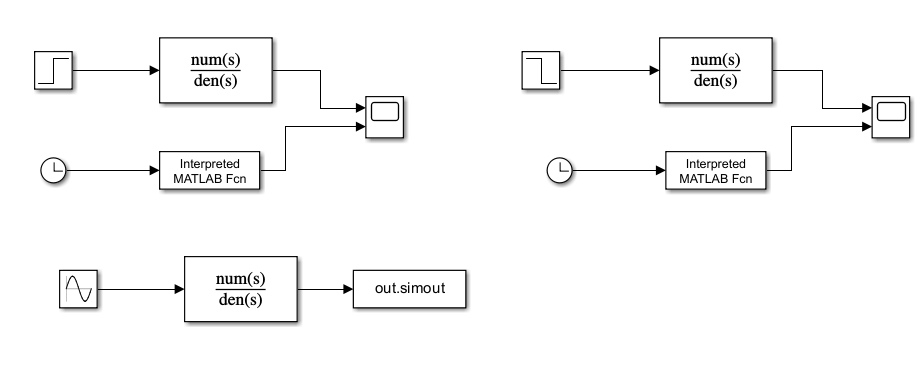
\includegraphics[width=0.8\textwidth]{images/schem.png}
    \caption{Схема моделирования в Simulink}
    \label{fig:2}
\end{figure}

\begin{figure}[H]
    \centering
    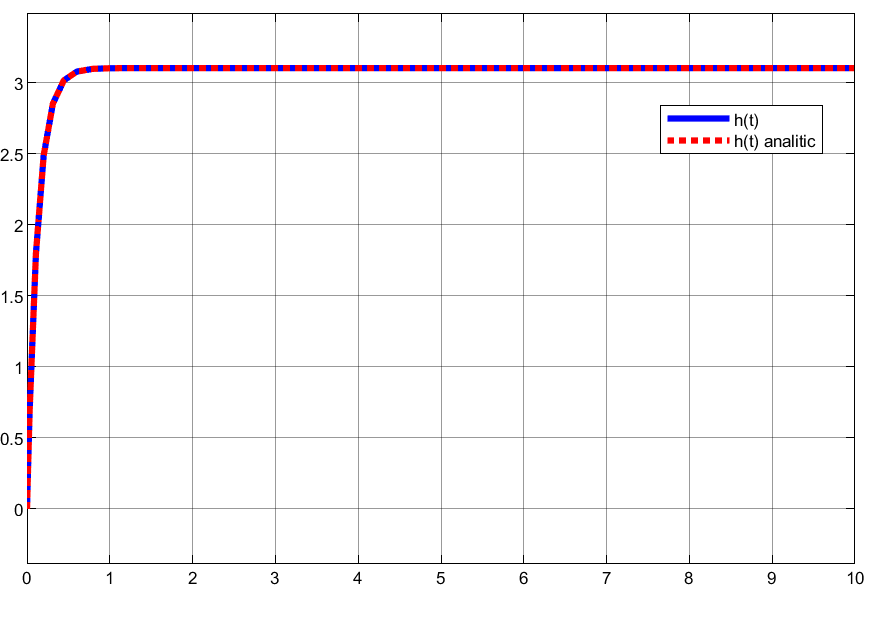
\includegraphics[width=0.8\textwidth]{images/h1.png}
    \caption{Переходная характеристика системы}
    \label{fig:2}
\end{figure}

\begin{figure}[H]
    \centering
    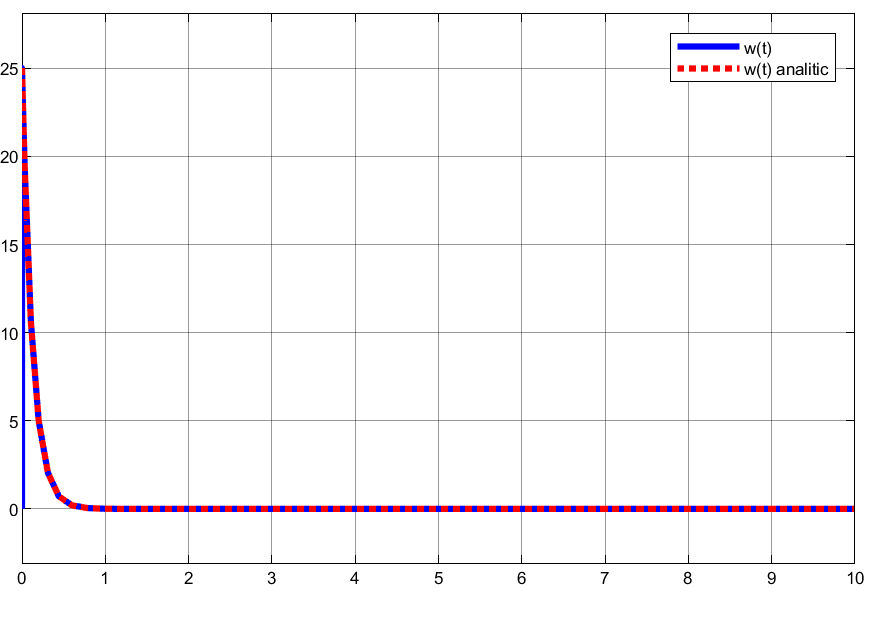
\includegraphics[width=0.8\textwidth]{images/w1.png}
    \caption{Весовая характеристика системы}
    \label{fig:2}
\end{figure}

\begin{figure}[H]
    \centering
    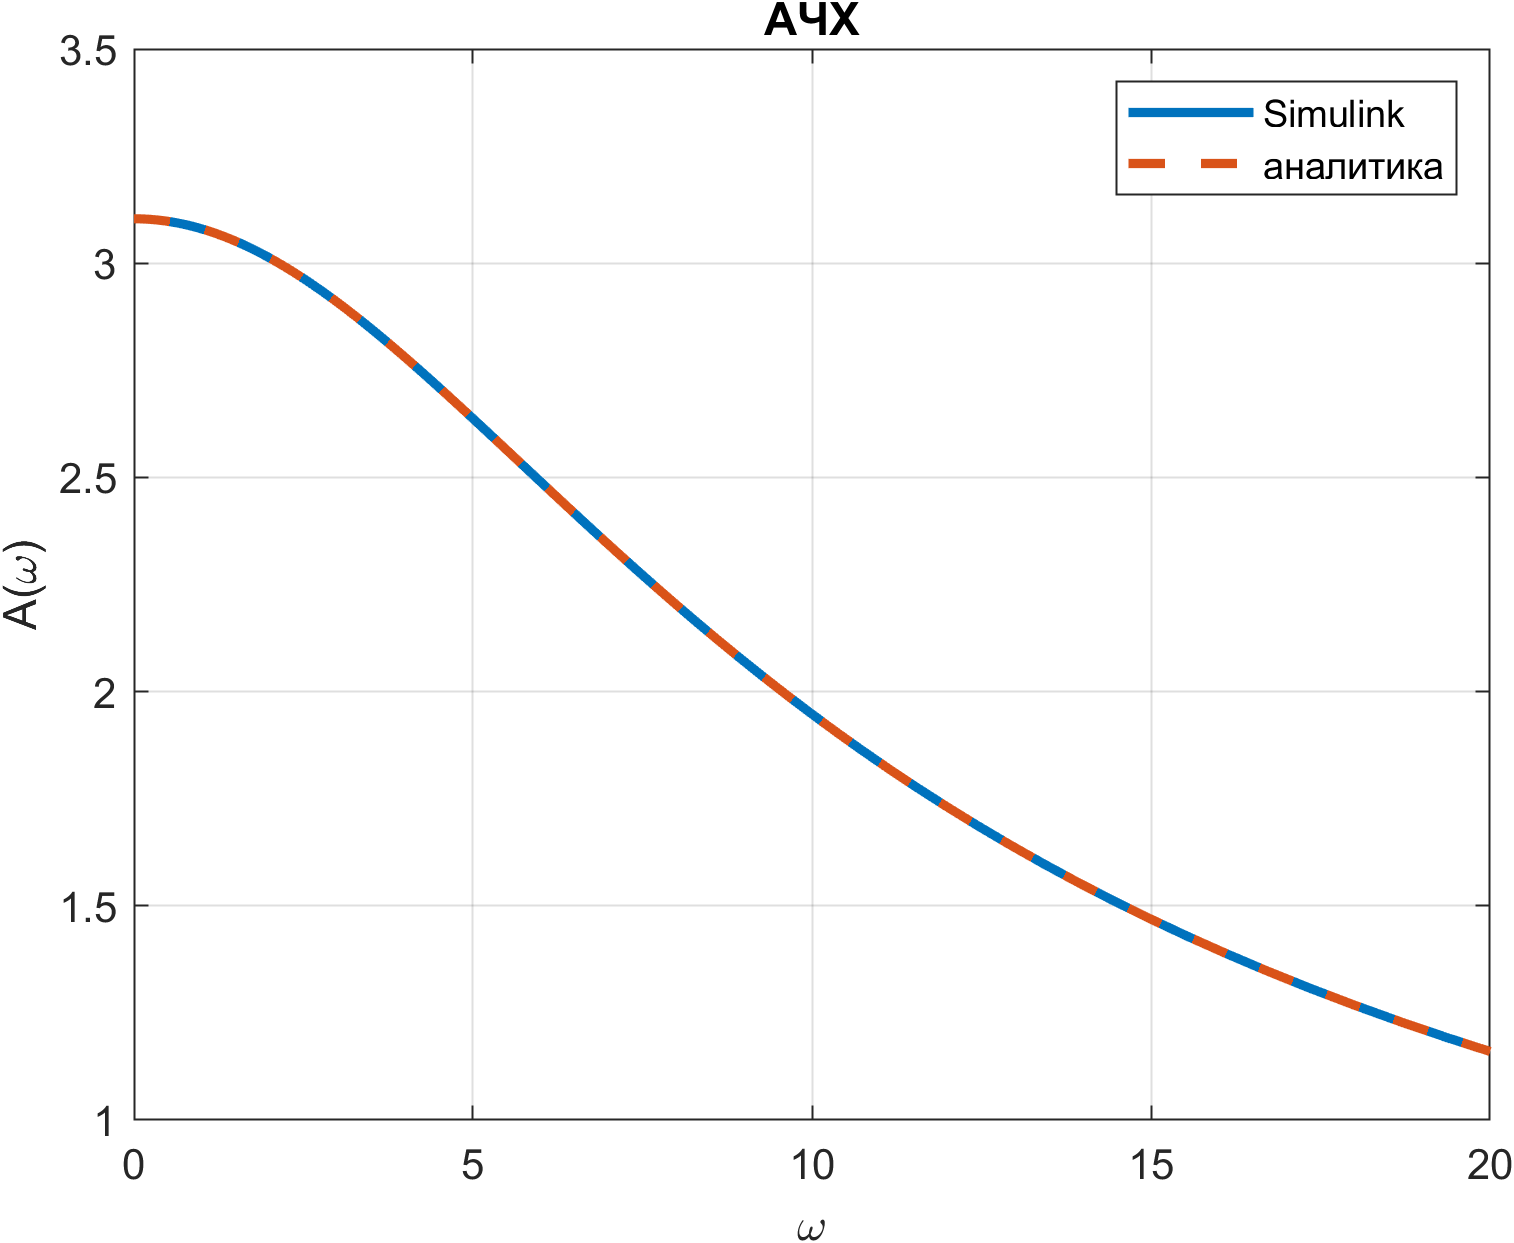
\includegraphics[width=0.8\textwidth]{images/ACH1.png}
    \caption{АЧХ системы}
    \label{fig:2}
\end{figure}

\begin{figure}[H]
    \centering
    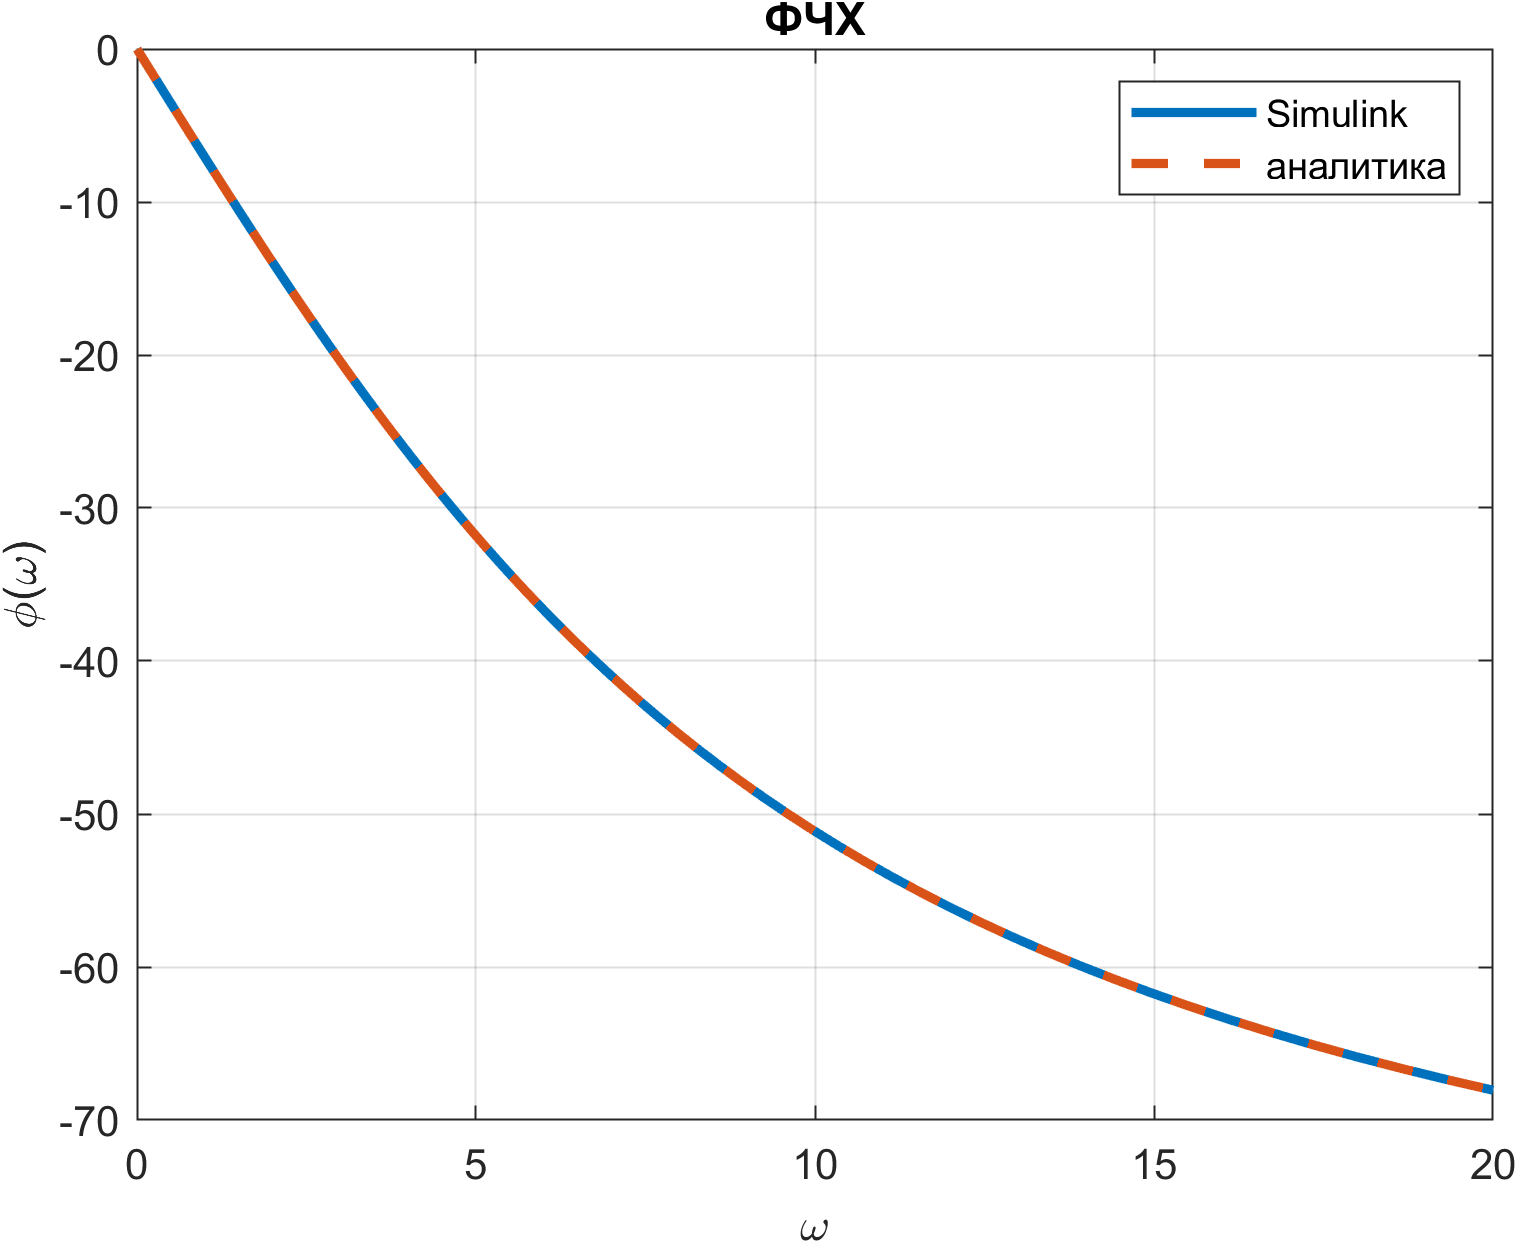
\includegraphics[width=0.8\textwidth]{images/FCH1.png}
    \caption{ФЧХ системы}
    \label{fig:2}
\end{figure}

\begin{figure}[H]
    \centering
    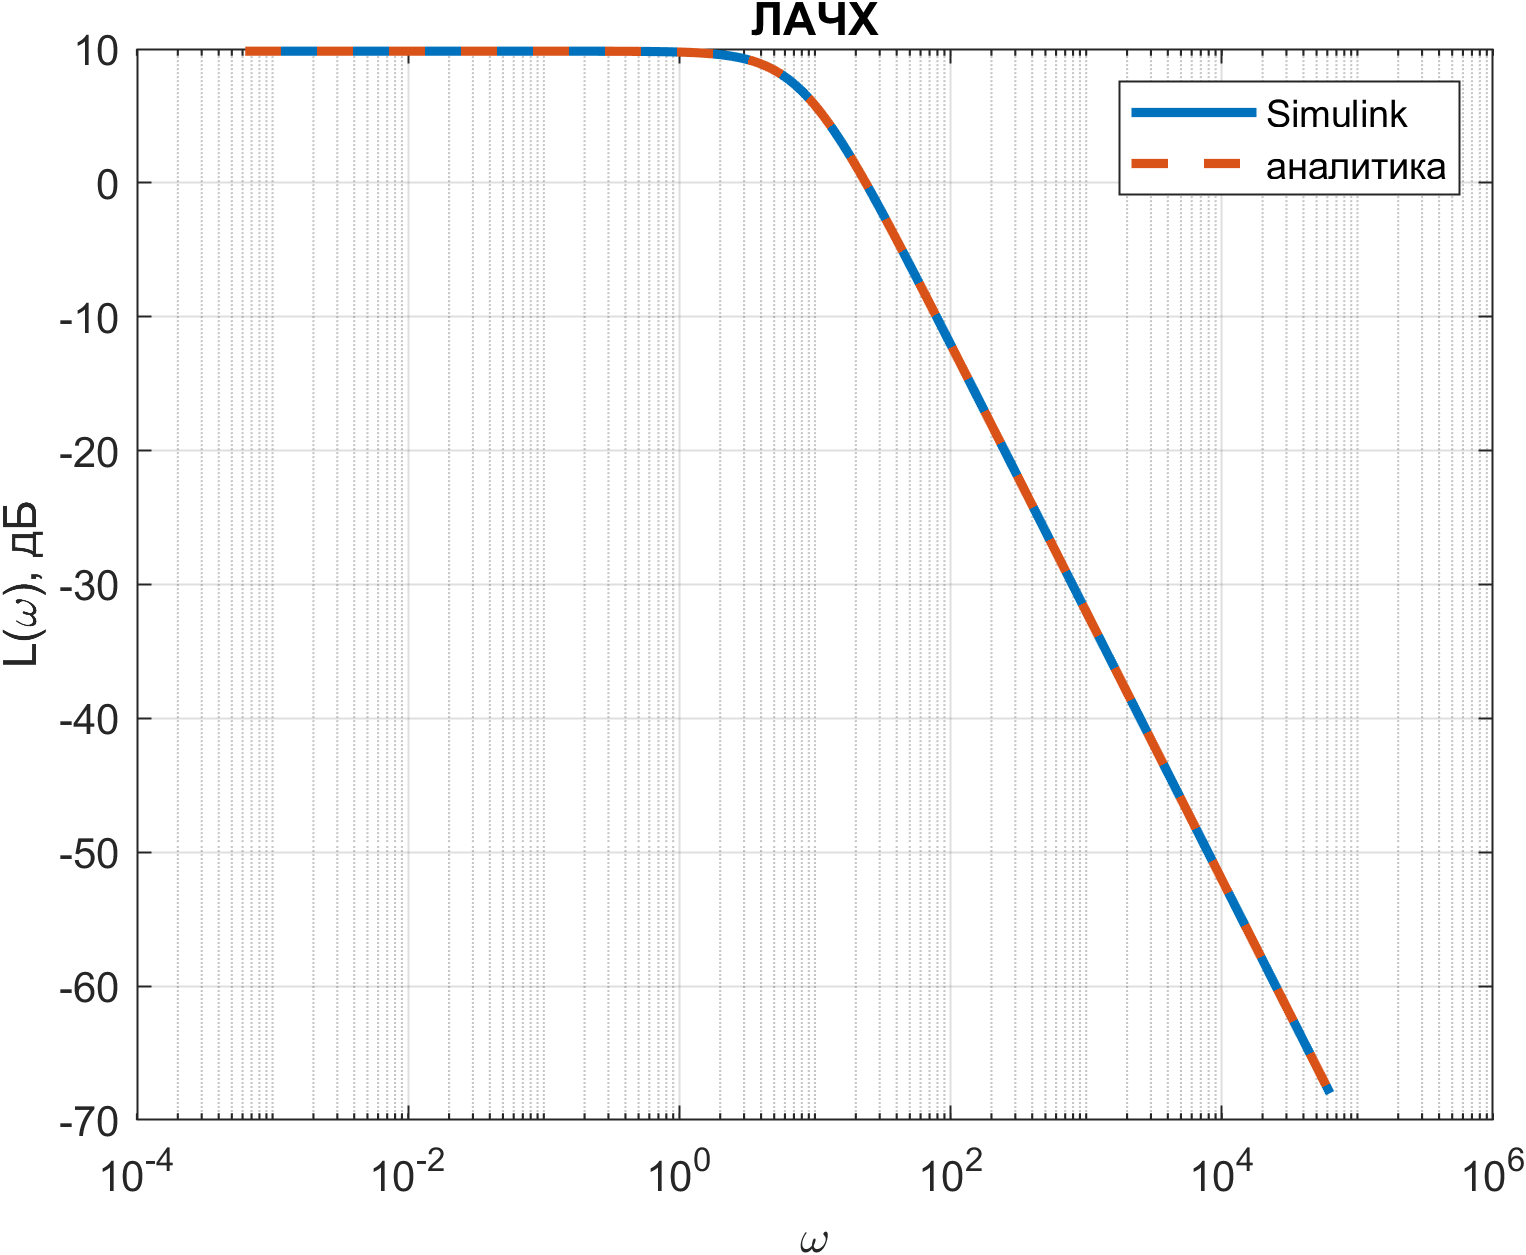
\includegraphics[width=0.8\textwidth]{images/LACH1.png}
    \caption{ЛАЧХ системы}
    \label{fig:2}
\end{figure}

\begin{figure}[H]
    \centering
    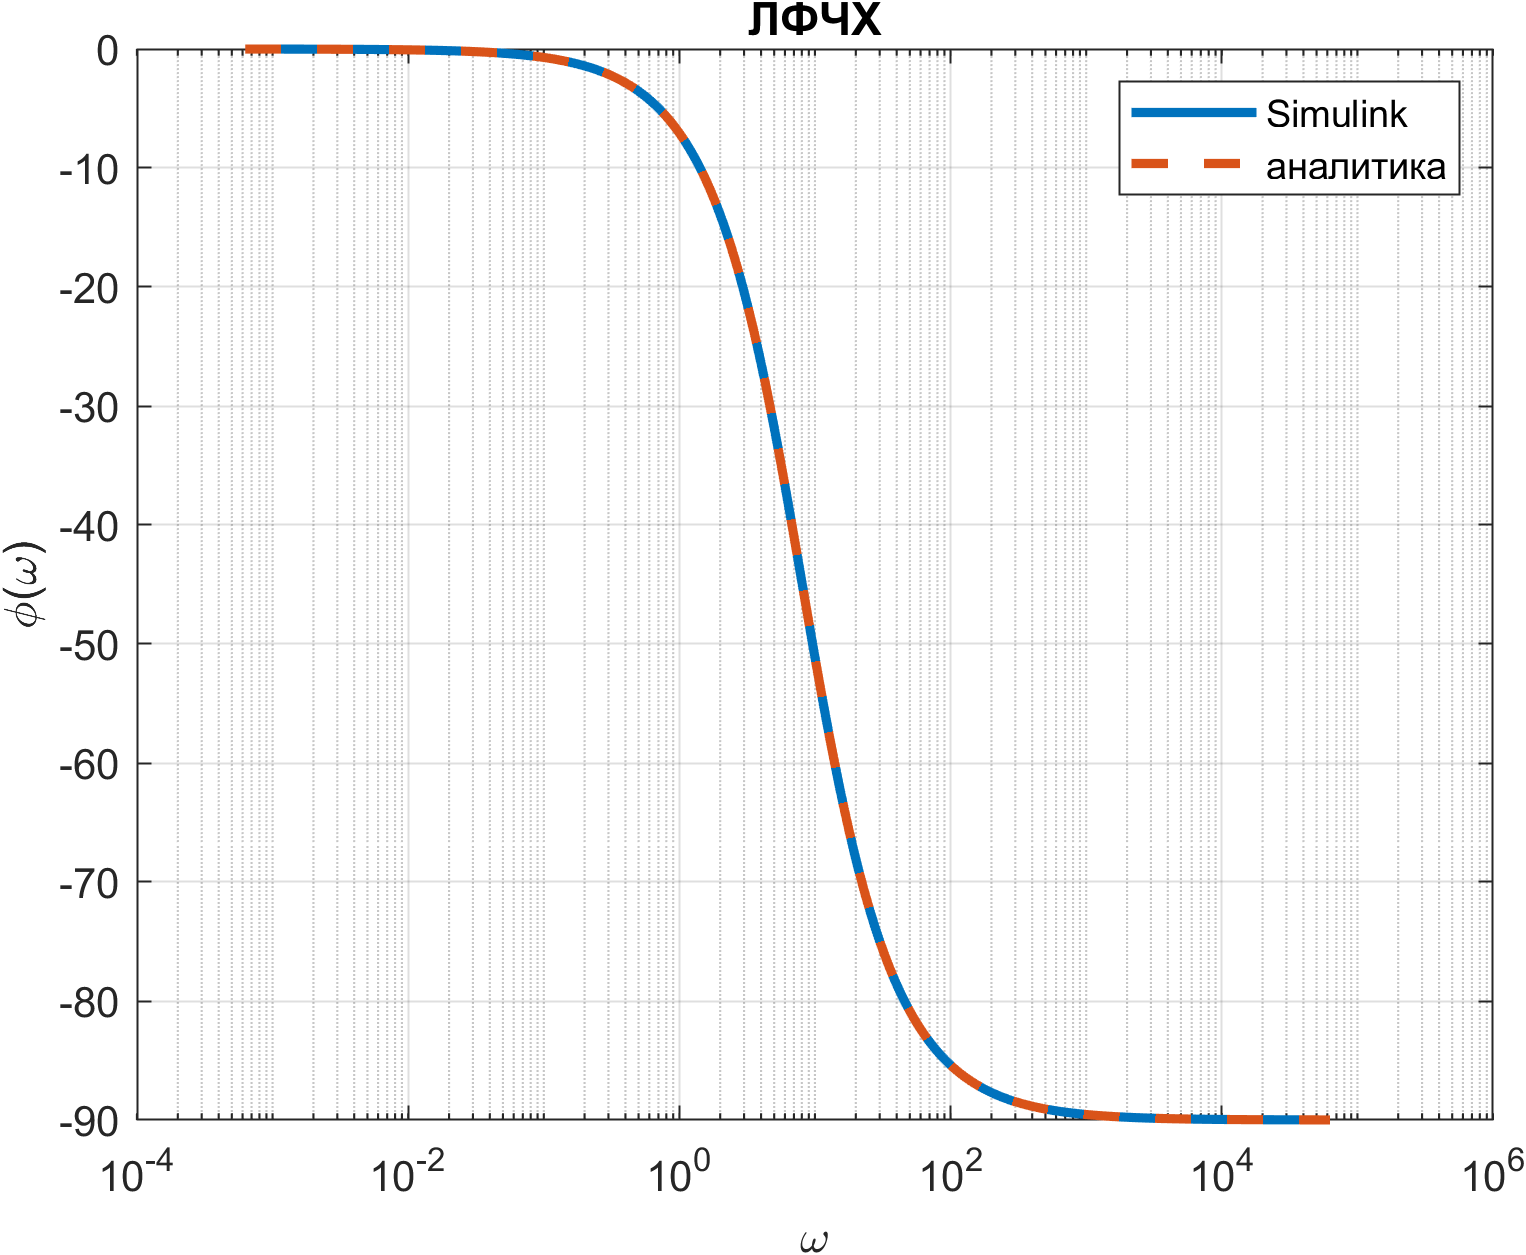
\includegraphics[width=0.8\textwidth]{images/LFCH1.png}
    \caption{ЛФЧХ системы}
    \label{fig:2}
\end{figure}

\newpage
\section{Двигатель постоянного тока с учетом индуктивности}
Добавим уравнения, учитывающие индуктивность
\[
J\dot{\omega} = M, \quad M = k_mI, \quad I = \frac{U + \epsilon}{R}, \quad \epsilon = \epsilon_i + \epsilon_s, \quad \epsilon_i = -k_e\omega, \quad \epsilon_s = -\L\dot{I}
\]
\[
\dot{\omega} = \frac{k_m I}{J} \qquad \dot{I} = \frac{U}{L} - \frac{k_e}{L}\omega -\frac{R}{L}I 
\]
\[
\frac{L}{R}\ddot{\omega} + \dot{\omega} + \frac{k_m k_e}{JR}\omega = \frac{k_m}{JR}U
\]

\[
T_m = \frac{JR}{k_m k_e}, \qquad T_e = \frac{L}{R}, \qquad \frac{1}{k_e}= K
\]
\[
T_m T_e\ddot{\omega} + T_m \dot{\omega} + 1 = K U
\]
Применив преобразование Лапласа
\[
W(s) = \frac{K}{T_m T_e s^2 + T_m s + 1}
\]
Пусть \(T = \sqrt{T_e T_m}\), тогда \(\xi = \frac{\sqrt{T_m T_e}}{2T_e}\). 
\[
W(s) = \frac{K}{T^2 s^2 + 2\xi T s + 1}
\]
При \(\xi > 1\), это 
апериодическое звено 2-го порядка. При \(\xi < 1\), это колебательное звено.

Рассмотрим данные значения
\[
k_m = 0.3222, \qquad k_e = 0.3222, \qquad J = 0.0028, \qquad R = 4.6013, \qquad L = 1.1319
\]
\[
T_m = 0,1241 \qquad T_e = 0,2460 \qquad \xi = 0,3551
\]
Таким образом моделируемая система - колебательная. Выведем аналитическое представление передаточной и весовой функции.
\[
s_{1,2} = \frac{-2\xi T \pm \sqrt{4\xi^2T^2 - 4T^2}}{2T^2} = \frac{-\xi \pm \sqrt{\xi^2 - 1}}{T}
\]
\[
\sigma_{\text{д}} = \frac{\xi}{T} \qquad \omega_{\text{д}} = \frac{\sqrt{1 - \xi^2}}{T} \qquad s_{1,2} = \sigma_{\text{д}} \pm i\omega_{\text{д}}
\]

\[
W(s) = \frac{K}{T^2(s+\sigma_{\text{д}} - i\omega_{\text{д}})(s+\sigma_{\text{д}} + i\omega_{\text{д}})} = \frac{K}{T^2}\frac{1}{(s+\sigma_{\text{д}})^2 + \omega_{\text{д}}^2}
\]
Применим преобразование Лапласа
\[
\omega (t) = \frac{Ke^{-\sigma_{\text{д}}t}}{T\sqrt{1-\xi^2}}sin(\omega_{\text{д}}t)
\]
\[
h(t) = K\left(1 - \frac{e^{-\sigma_{\text{д}}t}}{\sqrt{1-\xi^2}}sin(\omega_{\text{д}}t + arccos(\xi))\right)
\]
Получим частотные характеристики. Подставим $s = i\omega$:
\[
W(i\omega) = \frac{K}{1 - T^2\omega^2 + 2i\xi T\omega}
= \frac{K(1 - T^2\omega^2)}{(1 - T^2\omega^2)^2 + 4\xi^2T^2\omega^2}
- i\,\frac{2K\xi T\omega}{(1 - T^2\omega^2)^2 + 4\xi^2T^2\omega^2}
\]
Амплитудно-частотная характеристика равна модулю $W(i\omega)$
\[
A(\omega) = |W(i\omega)| = \frac{K}{\sqrt{(1 - T^2\omega^2)^2 + 4\xi^2T^2\omega^2}}
\]
Фазо-частотная характеристика равна аргументу $W(i\omega)$. Так как знаменатель комплексный, а вещественная часть меняет знак при $\omega = 1/T$, аргумент записывается кусочно, чтобы фаза была непрерывной и менялась от $0$ до $-\pi$
\[
\varphi(\omega) =
\begin{cases}
-\operatorname{arctg}\dfrac{2\xi T\omega}{1 - T^2\omega^2}, & \omega < \dfrac{1}{T},\\[3mm]
-\dfrac{\pi}{2}, & \omega = \dfrac{1}{T},\\[3mm]
-\pi - \operatorname{arctg}\dfrac{2\xi T\omega}{1 - T^2\omega^2}, & \omega > \dfrac{1}{T}.
\end{cases}
\]
Логарифмические характеристики
\[
L(\omega) = 20\lg A(\omega) = 20\lg K - 10\lg\left[(1 - T^2\omega^2)^2 + 4\xi^2T^2\omega^2\right]
\]
ЛФЧХ совпадает с $\varphi(\omega)$, но строится в логарифмическом масштабе по оси частот.

\begin{figure}[H]
    \centering
    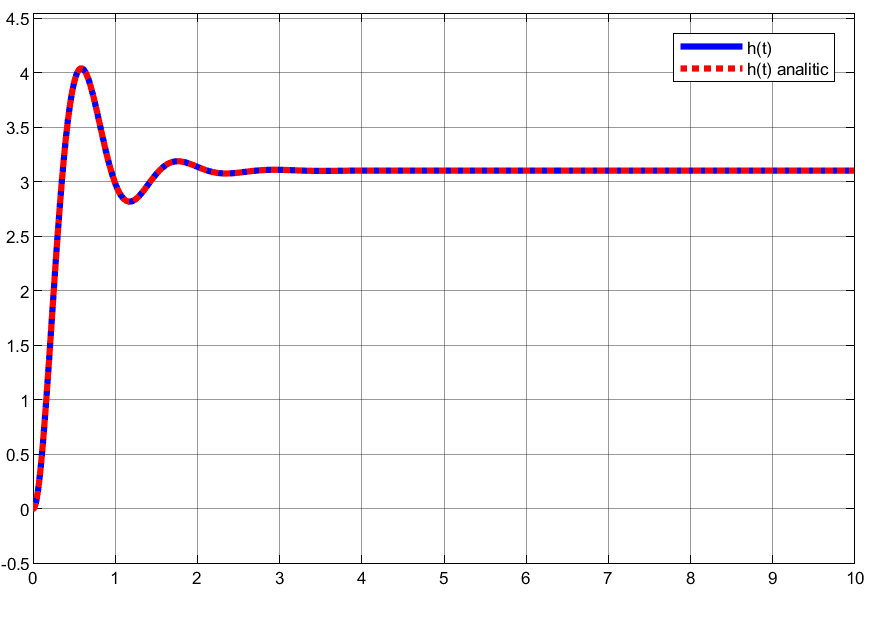
\includegraphics[width=0.8\textwidth]{images/h2.png}
    \caption{Переходная характеристика системы}
    \label{fig:2}
\end{figure}

\begin{figure}[H]
    \centering
    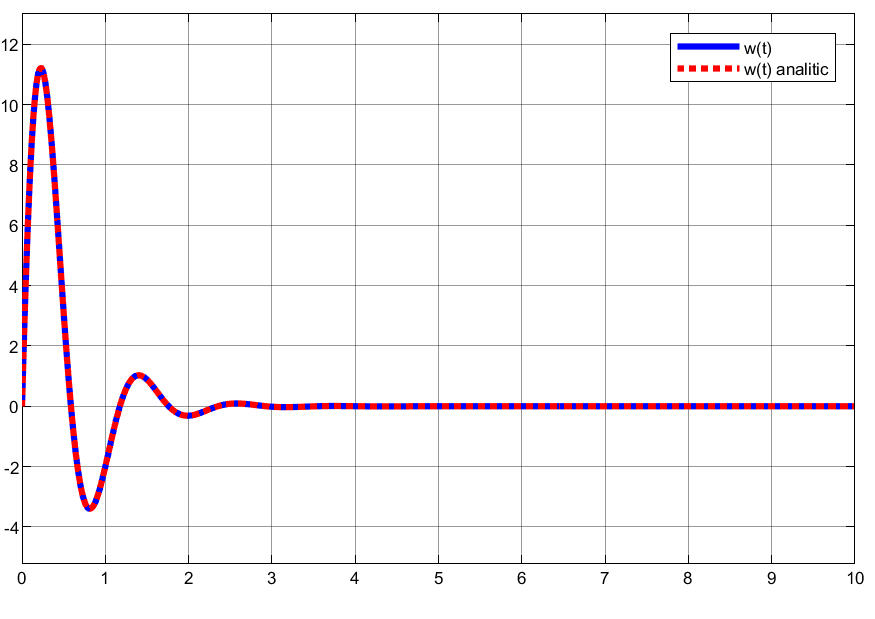
\includegraphics[width=0.8\textwidth]{images/w2.png}
    \caption{Весовая характеристика системы}
    \label{fig:2}
\end{figure}

\begin{figure}[H]
    \centering
    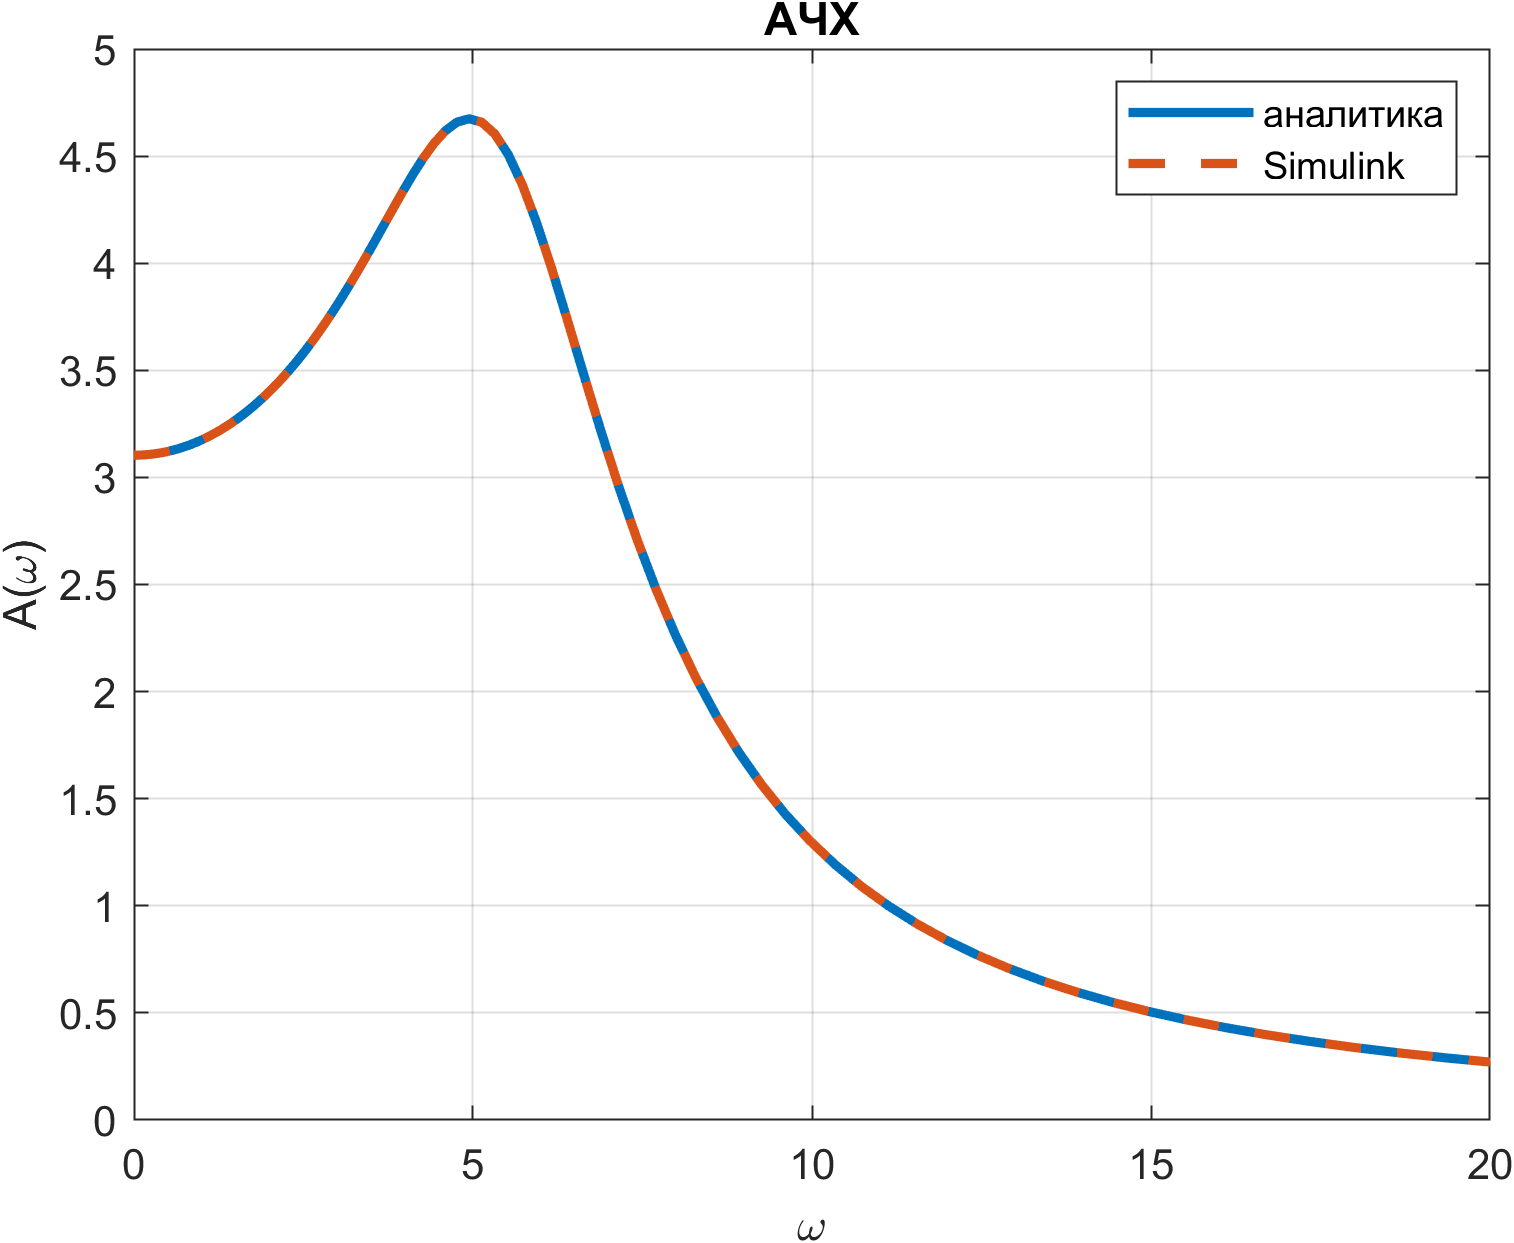
\includegraphics[width=0.8\textwidth]{images/ACH2.png}
    \caption{АЧХ системы}
    \label{fig:2}
\end{figure}

\begin{figure}[H]
    \centering
    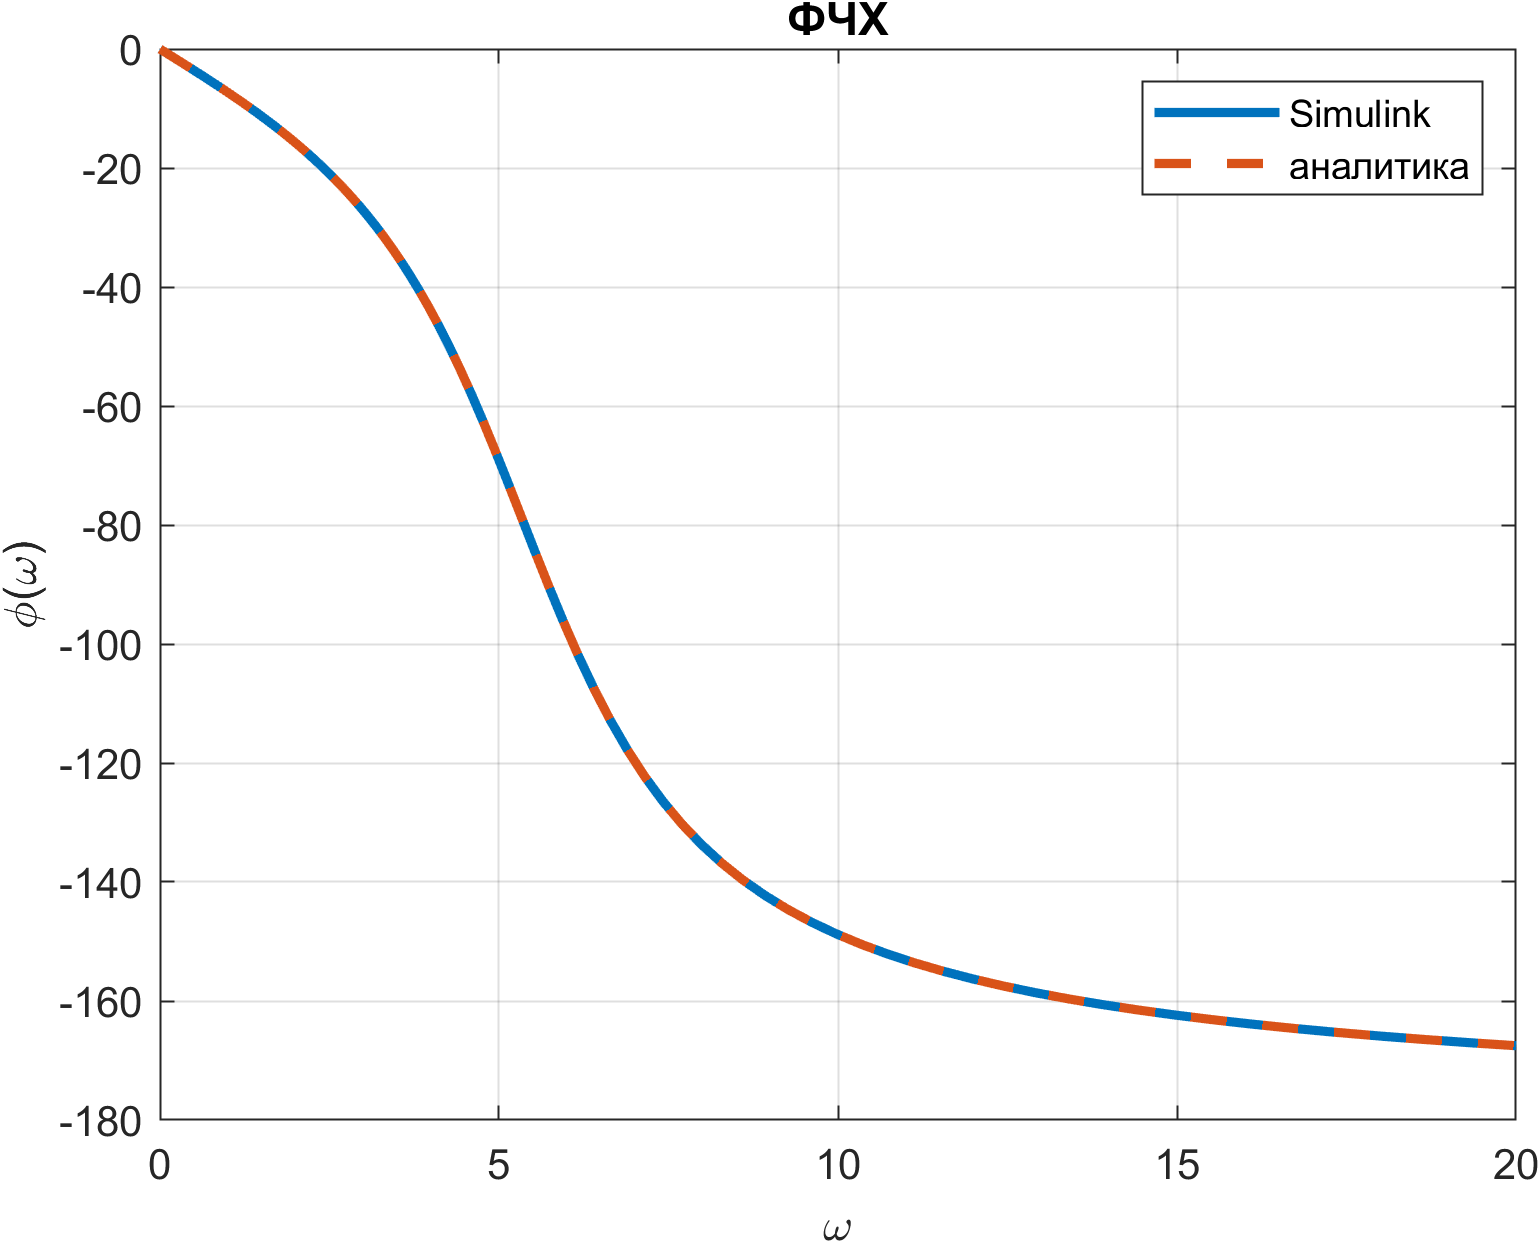
\includegraphics[width=0.8\textwidth]{images/FCH2.png}
    \caption{ФЧХ системы}
    \label{fig:2}
\end{figure}

\begin{figure}[H]
    \centering
    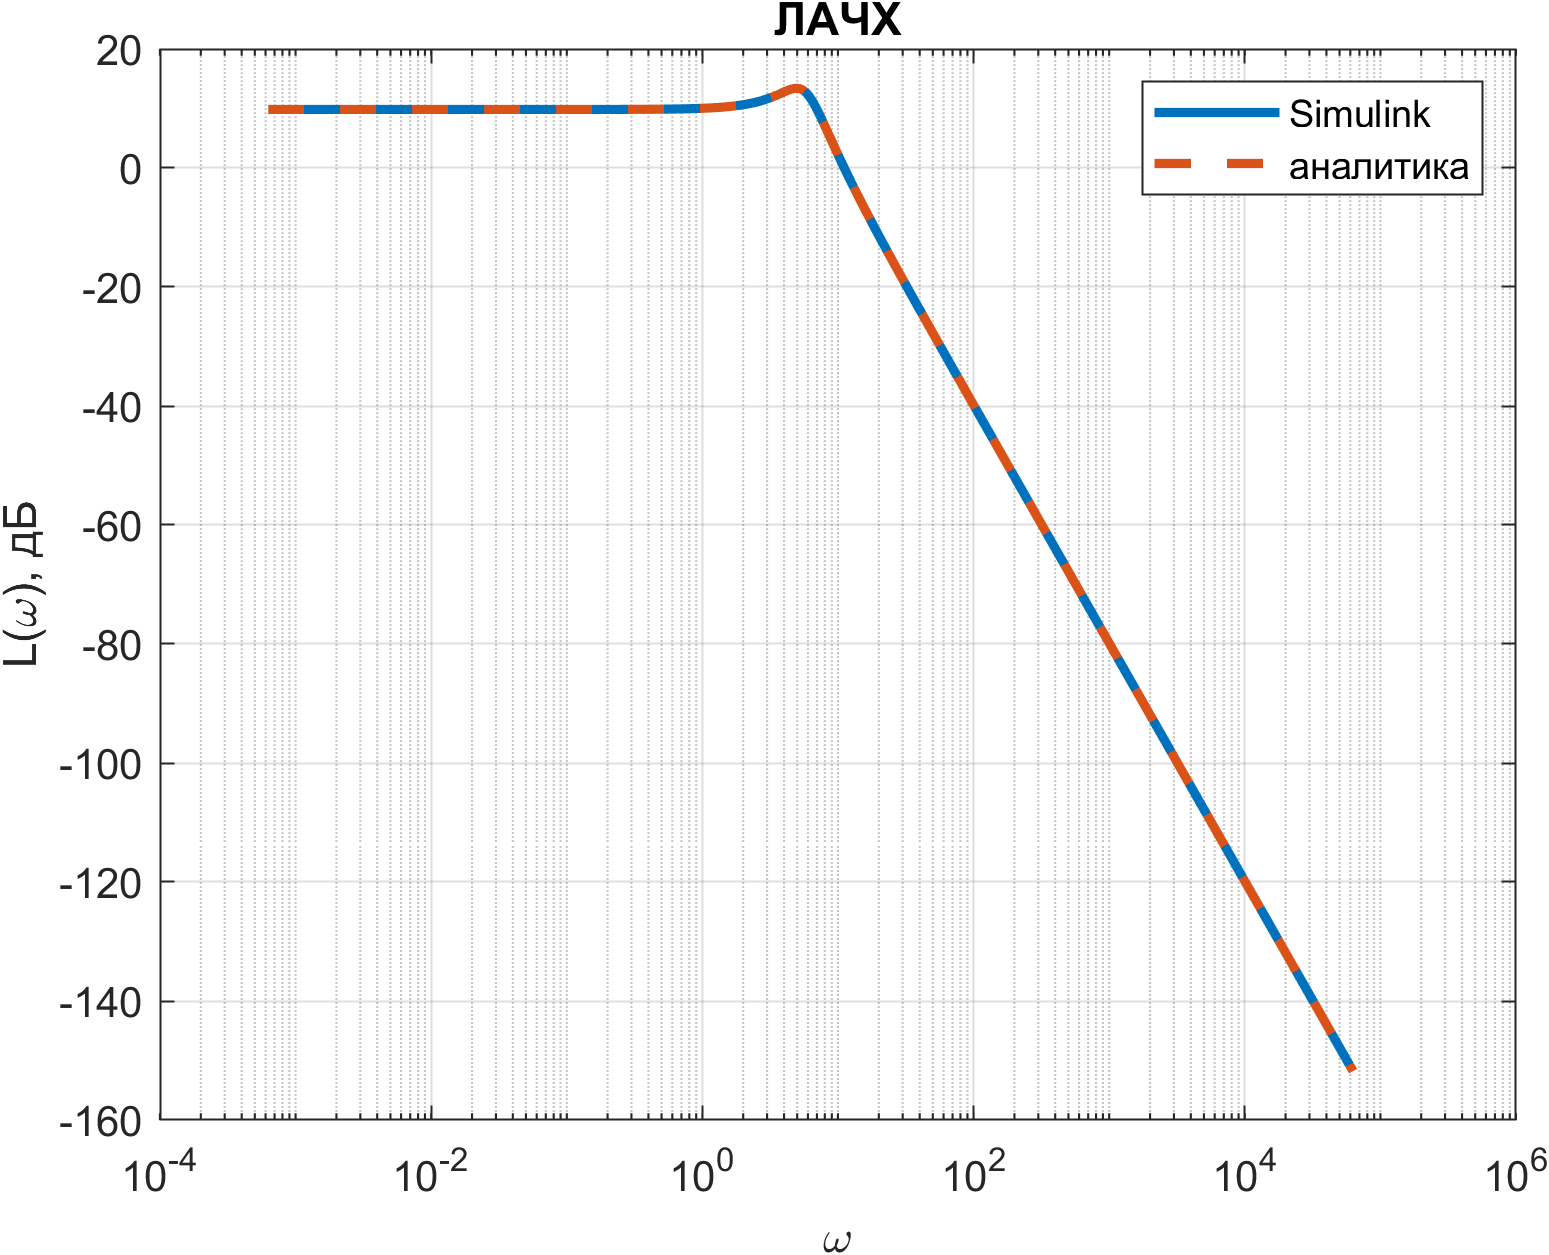
\includegraphics[width=0.8\textwidth]{images/LACH2.png}
    \caption{ЛАЧХ системы}
    \label{fig:2}
\end{figure}

\begin{figure}[H]
    \centering
    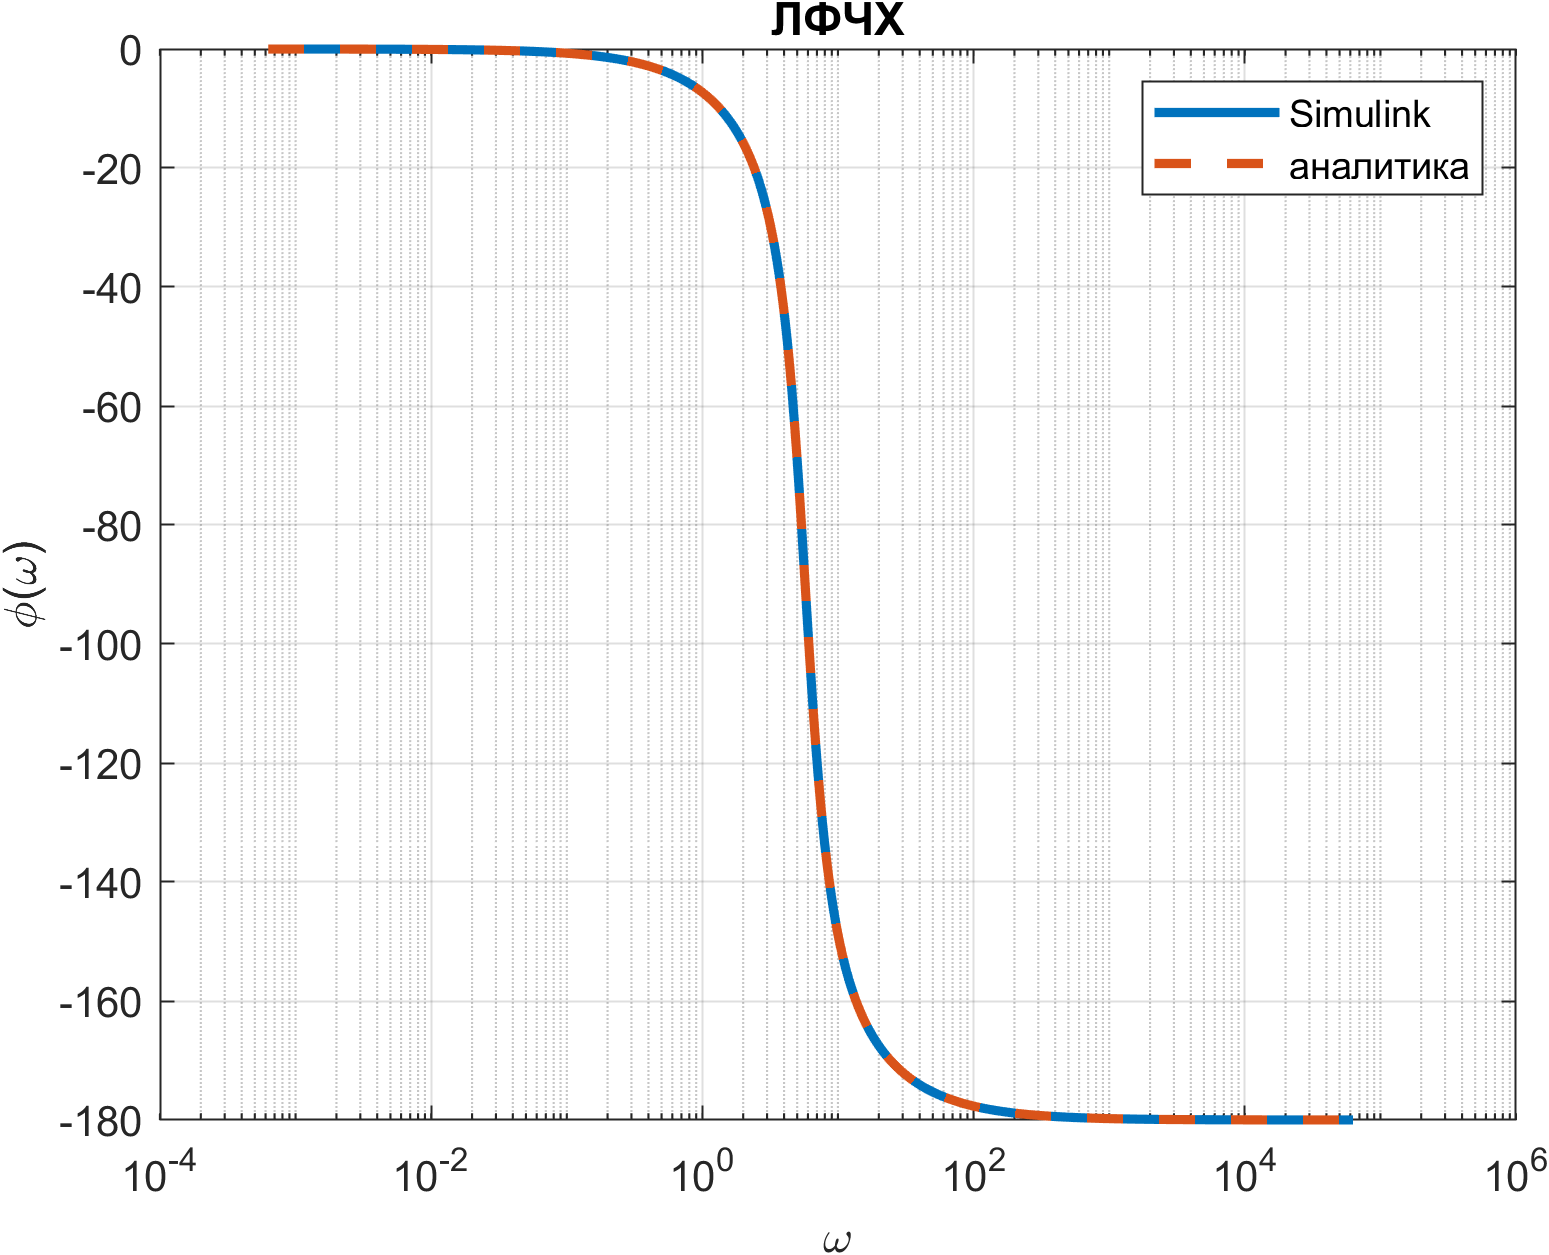
\includegraphics[width=0.8\textwidth]{images/LFCH2.png}
    \caption{ЛФЧХ системы}
    \label{fig:2}
\end{figure}    
\newpage

\section{Конденсатор}
Рассмотрим
\[
I = C\frac{dU}{dt}
\]
После преобразования лапласа
\[
W(s) = Cs
\]
Это идеальное дифференцирующее звено, где \(K = C\)
\[
\omega (t) = K \frac{d\delta (t)}{dt}
\]
\[
h(t) = K\delta (t)
\]
Получим частотные характеристики. Подставим $s = i\omega$:
\[
W(i\omega) = iK\omega
\]
Вещественная часть равна нулю, мнимая равна $K\omega$, поэтому
\[
A(\omega) = K\omega, \qquad \varphi(\omega) = \frac{\pi}{2}
\]
\[
L(\omega) = 20\lg K + 20\lg\omega
\]
ЛАЧХ представляет собой прямую с наклоном $+20$ дБ/дек, пересекающую ось $0$ дБ на частоте $\omega = 1/K$. Фаза не зависит от частоты.

Зададимся параметром \(C = 379\) мкФ и промоделируем систему

\begin{figure}[H]
    \centering
    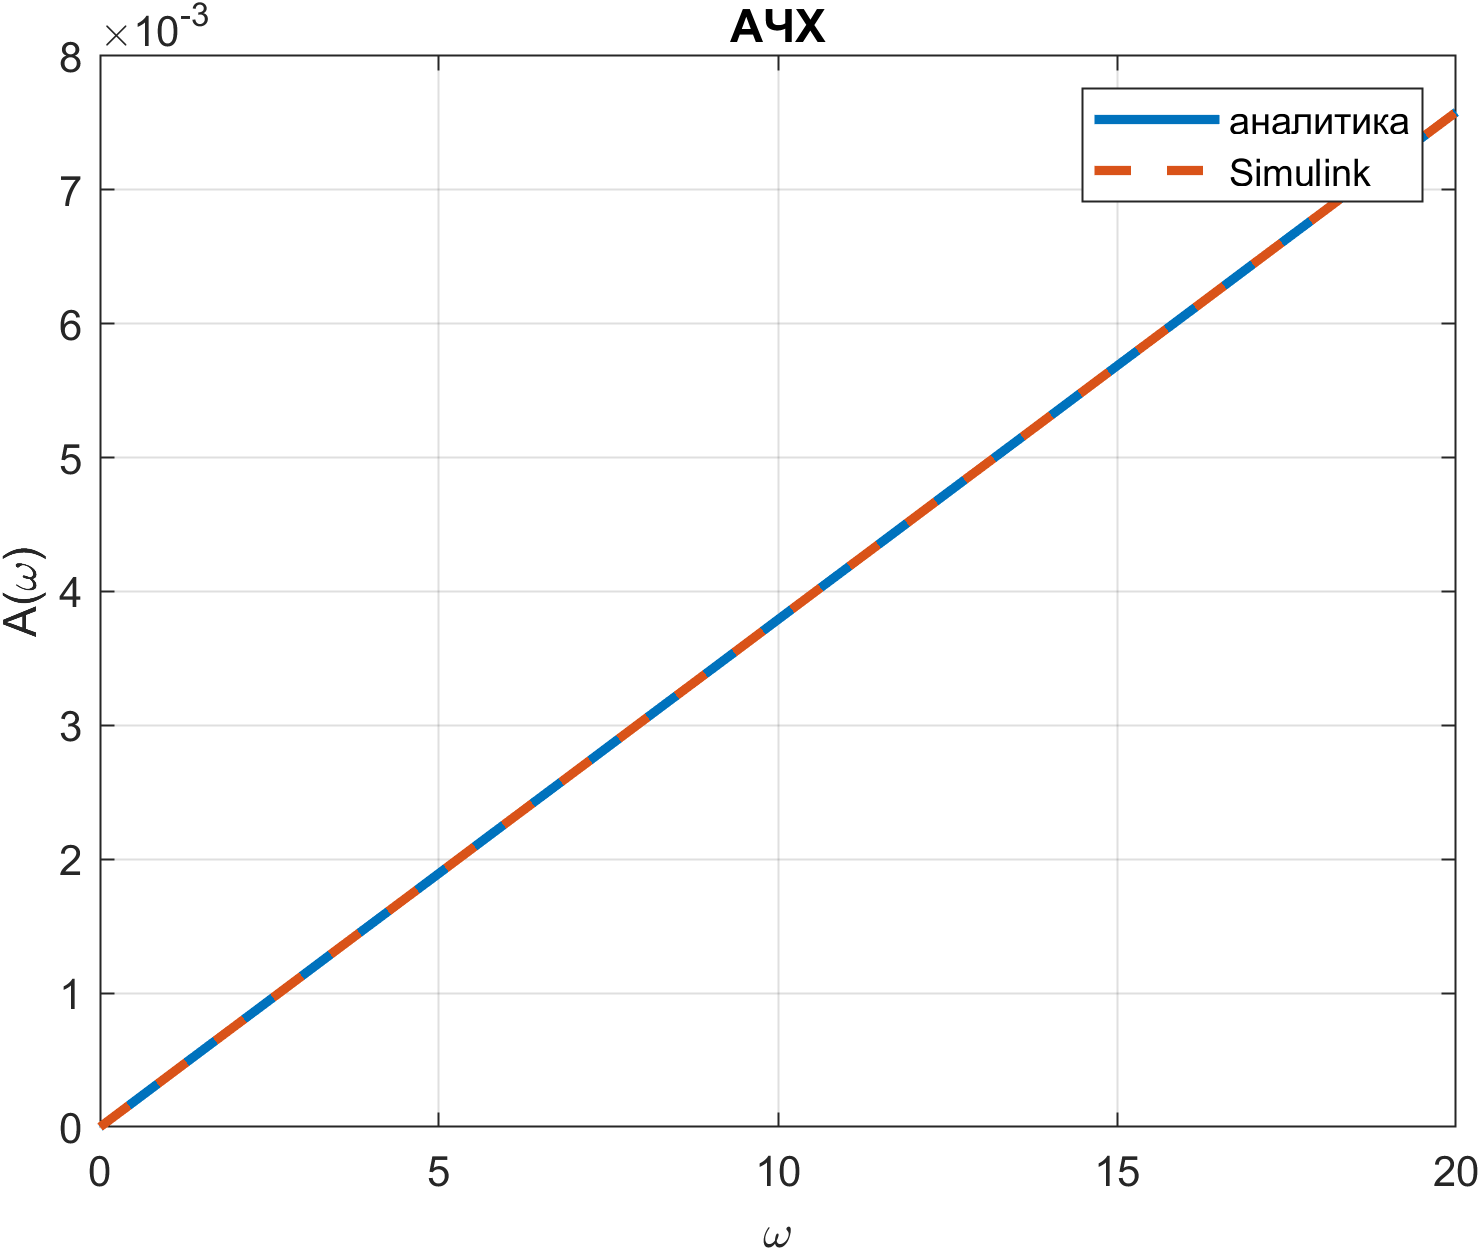
\includegraphics[width=0.8\textwidth]{images/ACH3.png}
    \caption{АЧХ системы}
    \label{fig:2}
\end{figure}

\begin{figure}[H]
    \centering
    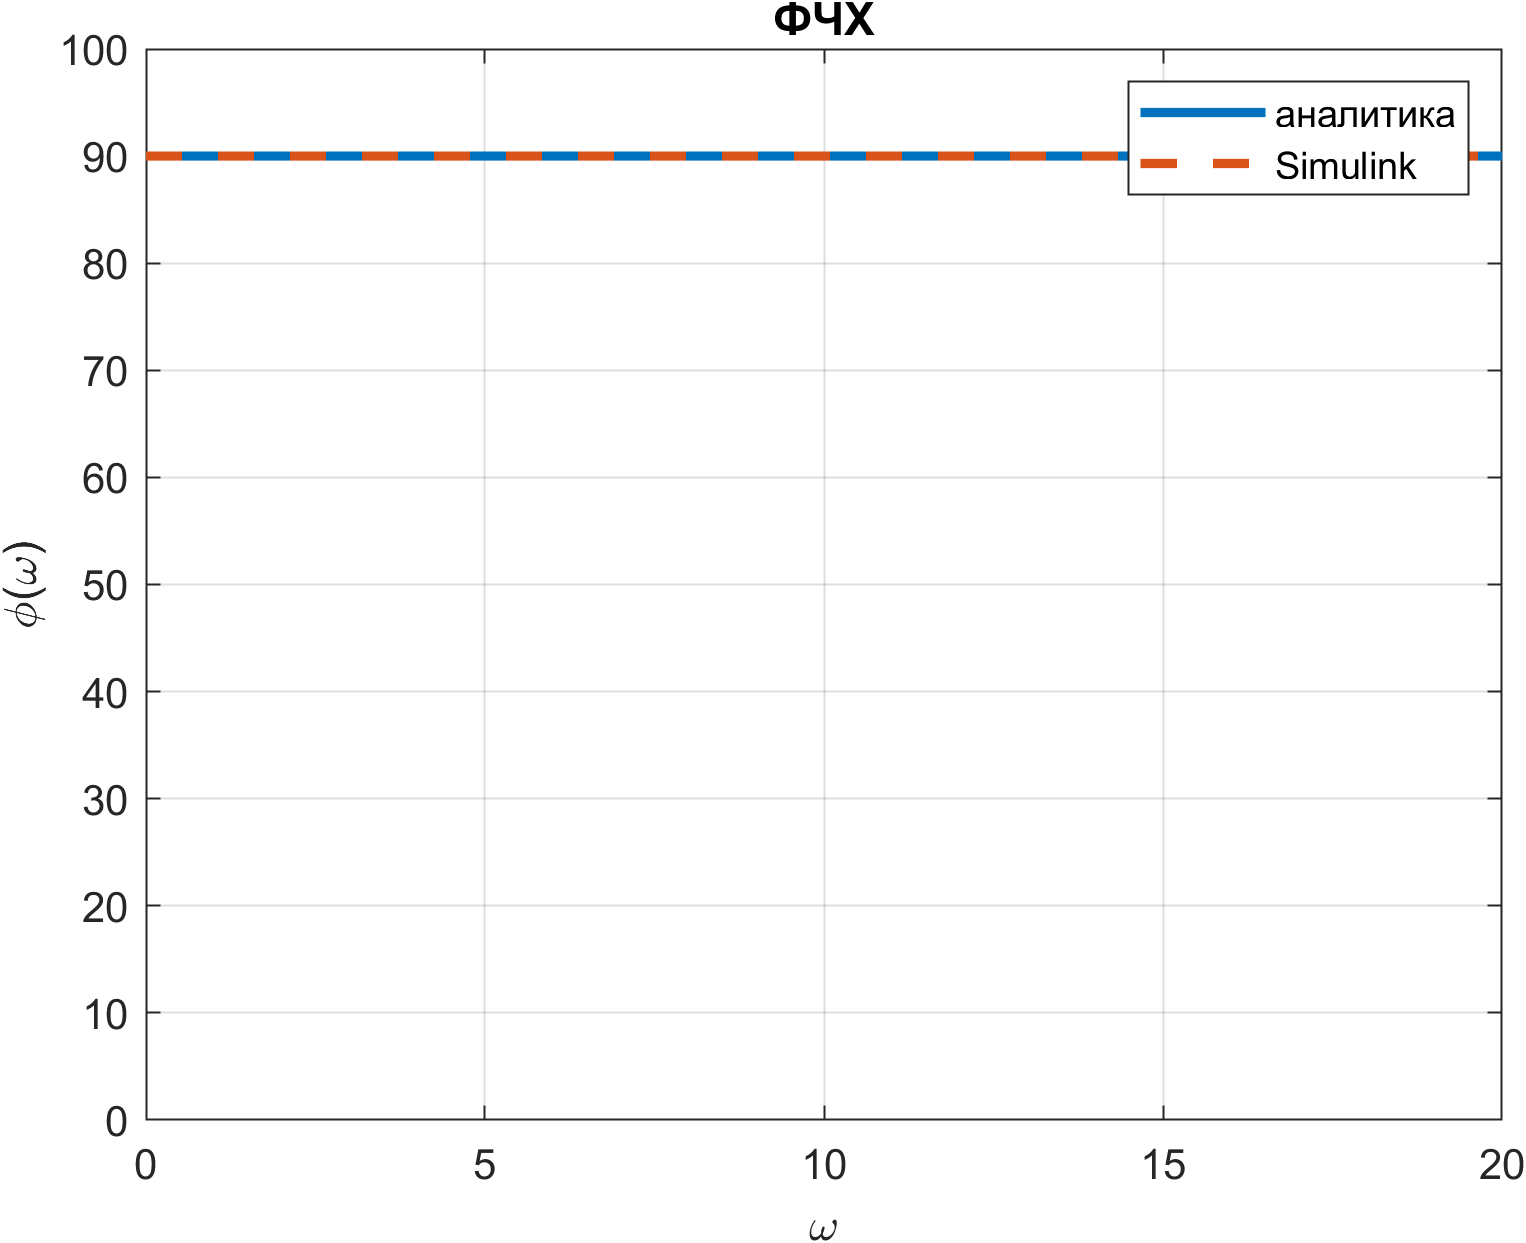
\includegraphics[width=0.8\textwidth]{images/FCH3.png}
    \caption{ФЧХ системы}
    \label{fig:2}
\end{figure}

\begin{figure}[H]
    \centering
    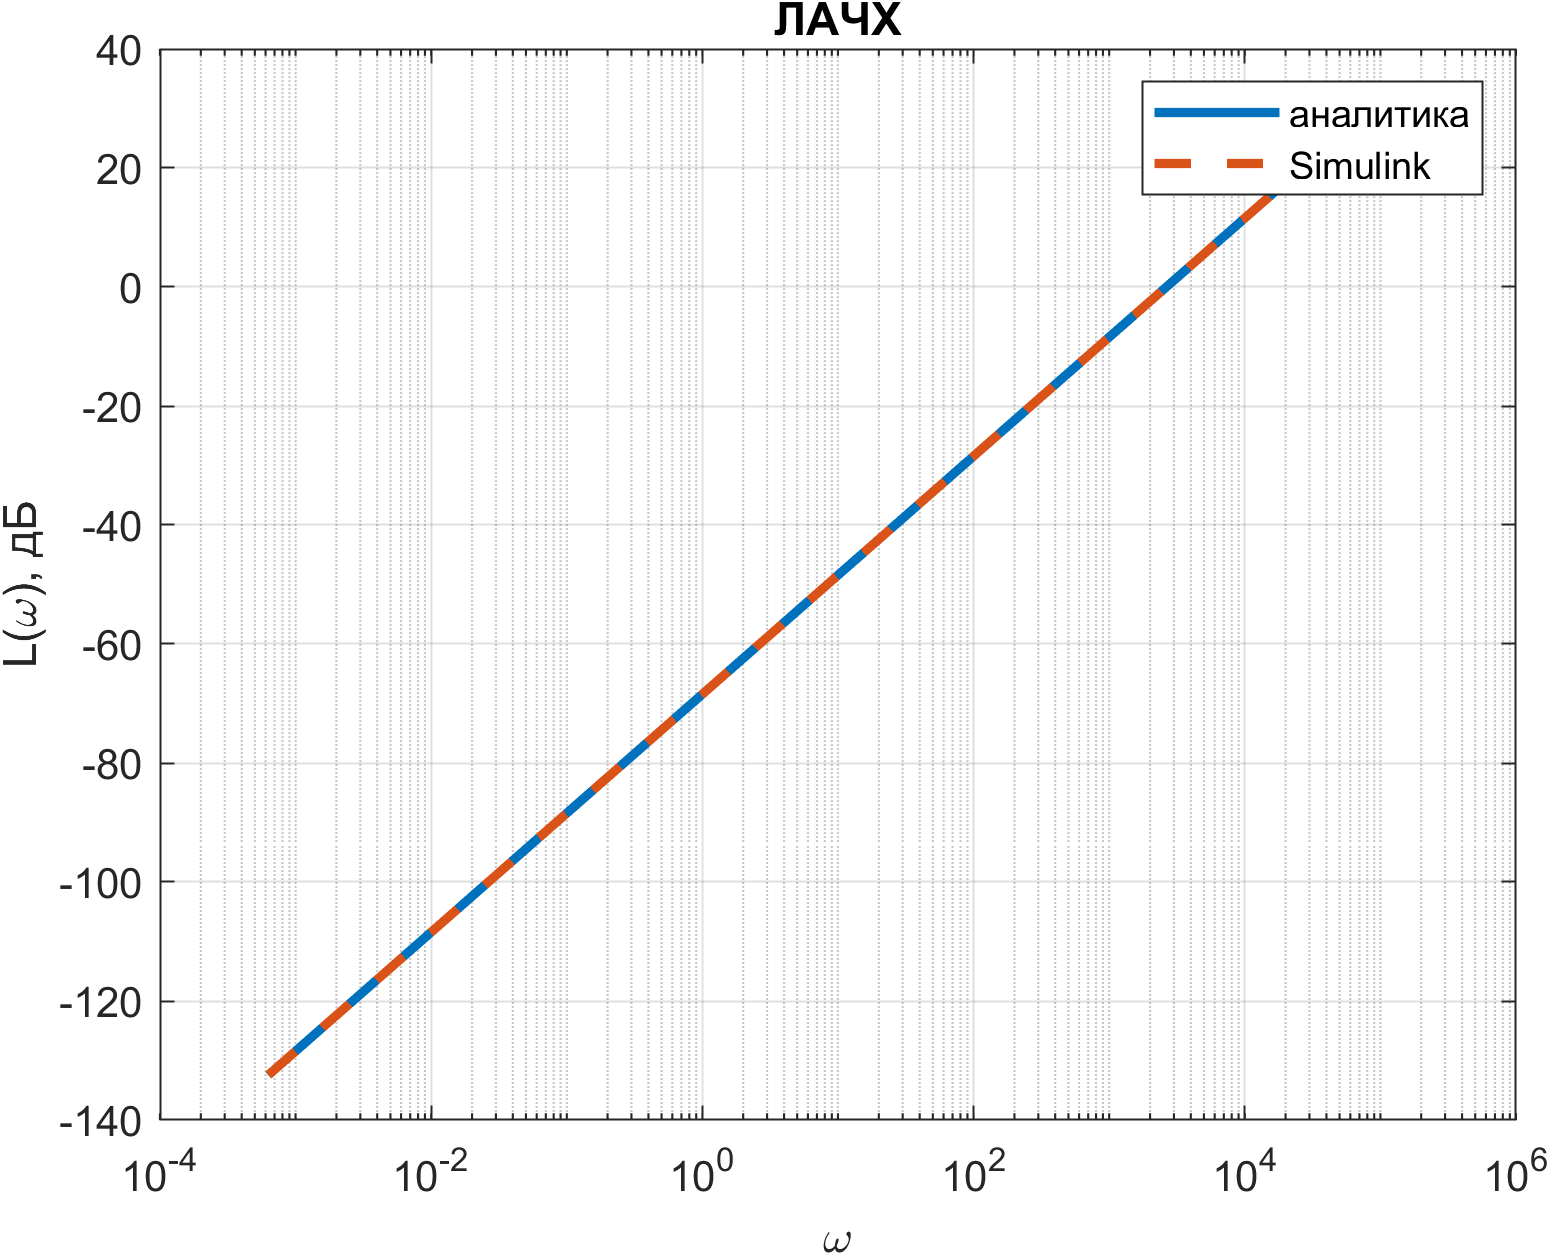
\includegraphics[width=0.8\textwidth]{images/LACH3.png}
    \caption{ЛАЧХ системы}
    \label{fig:2}
\end{figure}

\begin{figure}[H]
    \centering
    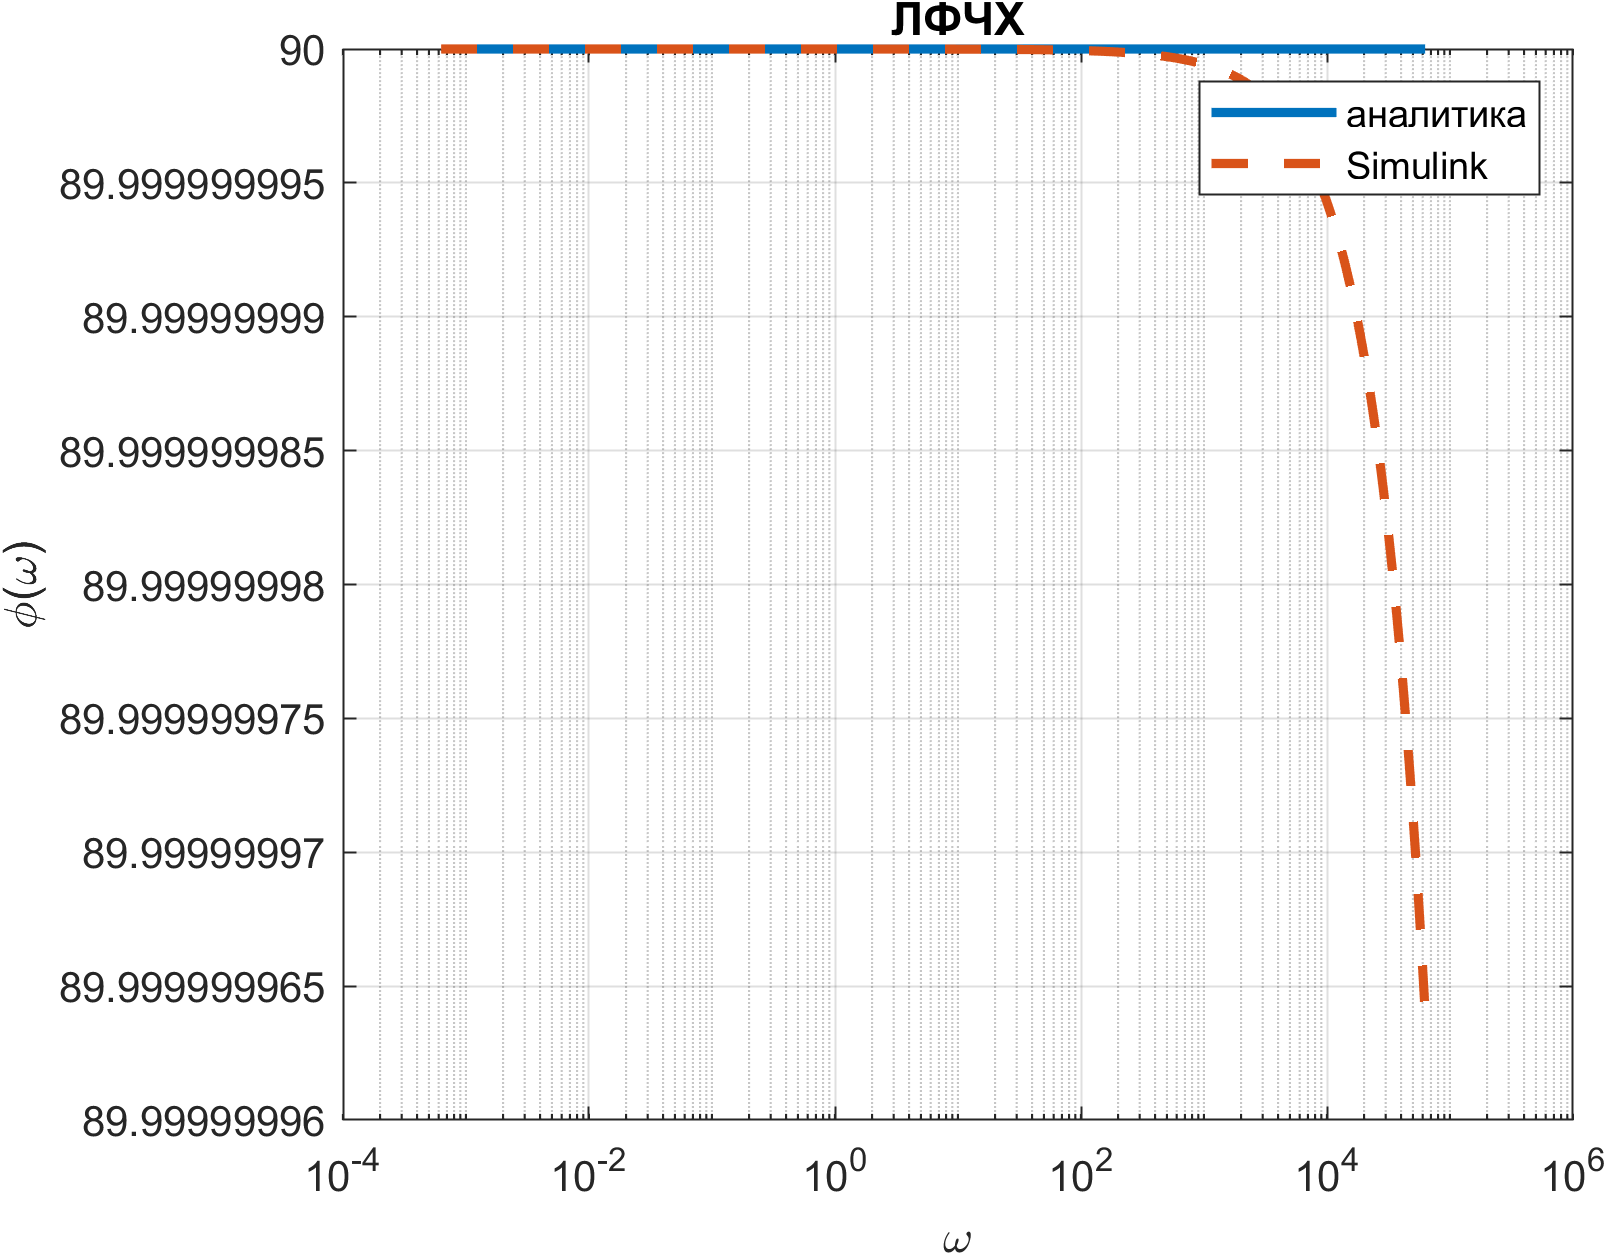
\includegraphics[width=0.8\textwidth]{images/LFCH3.png}
    \caption{ЛФЧХ системы}
    \label{fig:2}
\end{figure} 
На последнем графике имеется расхождение в симуляции и аналитическом представлении, это вызвано тем, что в simulink для моделирования использована
функция deriviative, которая аппроксимирует данное звено при помощи передаточной функции \(\frac{s}{cs +1}\), где с близко к нулю. Дельта функция и её производная - это обобщённые функции и их графики либо не существуют, либо строятся сложно.

\newpage
\section{Пружина}
Зададимся моделью пружинного маятника
\[
F_{\text{упр}} = -kx, \qquad F = ma
\]
Входом выступает внешняя сила, направленная соосно, выходом - положение маятника.

\[
F = F_{\text{упр}} + F_{\text{вн}} \rightarrow F_{\text{вн}} - kx = M\ddot{x}
\]
\[
M\ddot{x} + kx = F_{\text{вн}}
\]
Применим преобразование Лапласа
\[
W(s) = \frac{1}{Ms^2 + k}
\]
Это консервативное звено при
\[
K = \frac{1}{k}, \qquad T = \sqrt{\frac{M}{k}}, \qquad W(s) = \frac{K}{T^2s^2 + 1}
\]

Тогда весовая и переходная функции
\[
\omega(t) = \frac{K}{T} sin(\frac{t}{T})
\]
\[
h(t) = K\left(1 - cos(\frac{t}{T})\right)
\]
Получим частотные характеристики. Подставим $s = i\omega$:
\[
W(i\omega) = \frac{K}{1 - T^2\omega^2}
\]
Передаточная функция при $s = i\omega$ вещественна, поэтому
\[
A(\omega) = \frac{K}{|1 - T^2\omega^2|}, \qquad
\varphi(\omega) =
\begin{cases}
0, & \omega < \dfrac{1}{T},\\[3mm]
-\pi, & \omega > \dfrac{1}{T}.
\end{cases}
\]
\[
L(\omega) = 20\lg K - 20\lg\left|1 - T^2\omega^2\right|
\]

Зададимся значениеми 
\[
k = 140, \qquad M = 27
\]
И просимулируем систему
\newpage

\begin{figure}[H]
    \centering
    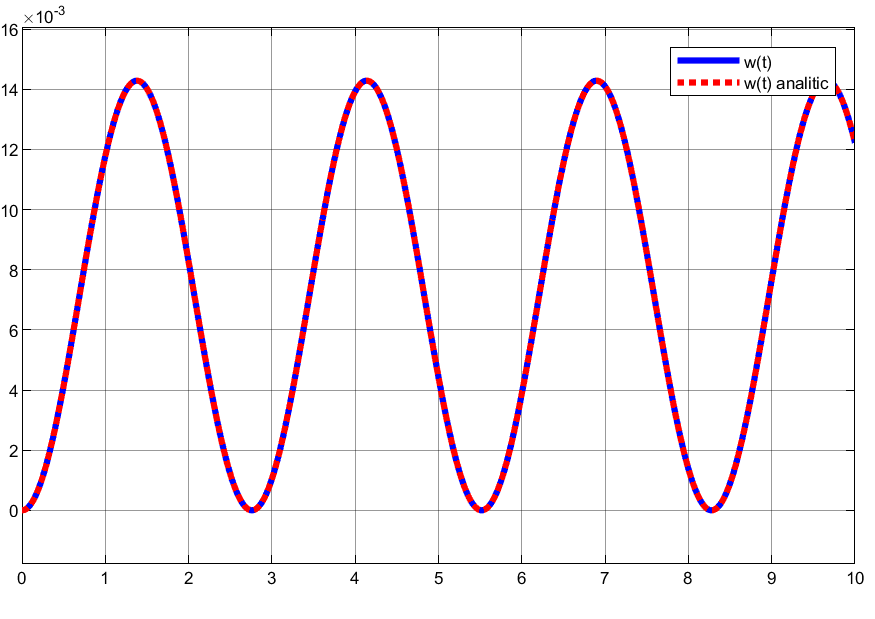
\includegraphics[width=0.8\textwidth]{images/w4.png}
    \caption{Переходная характеристика системы}
    \label{fig:2}
\end{figure}

\begin{figure}[H]
    \centering
    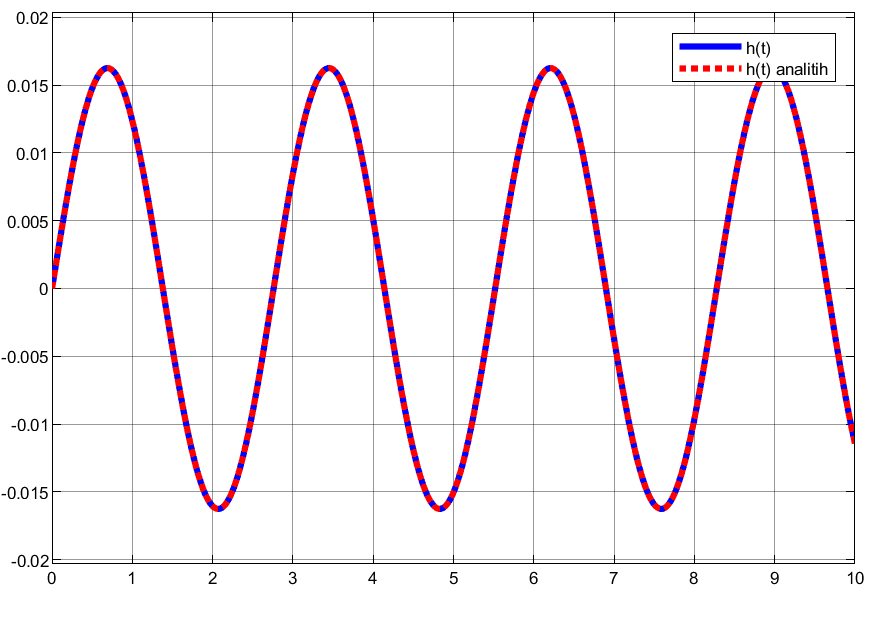
\includegraphics[width=0.8\textwidth]{images/h4.png}
    \caption{Весовая характеристика системы}
    \label{fig:2}
\end{figure}

\begin{figure}[H]
    \centering
    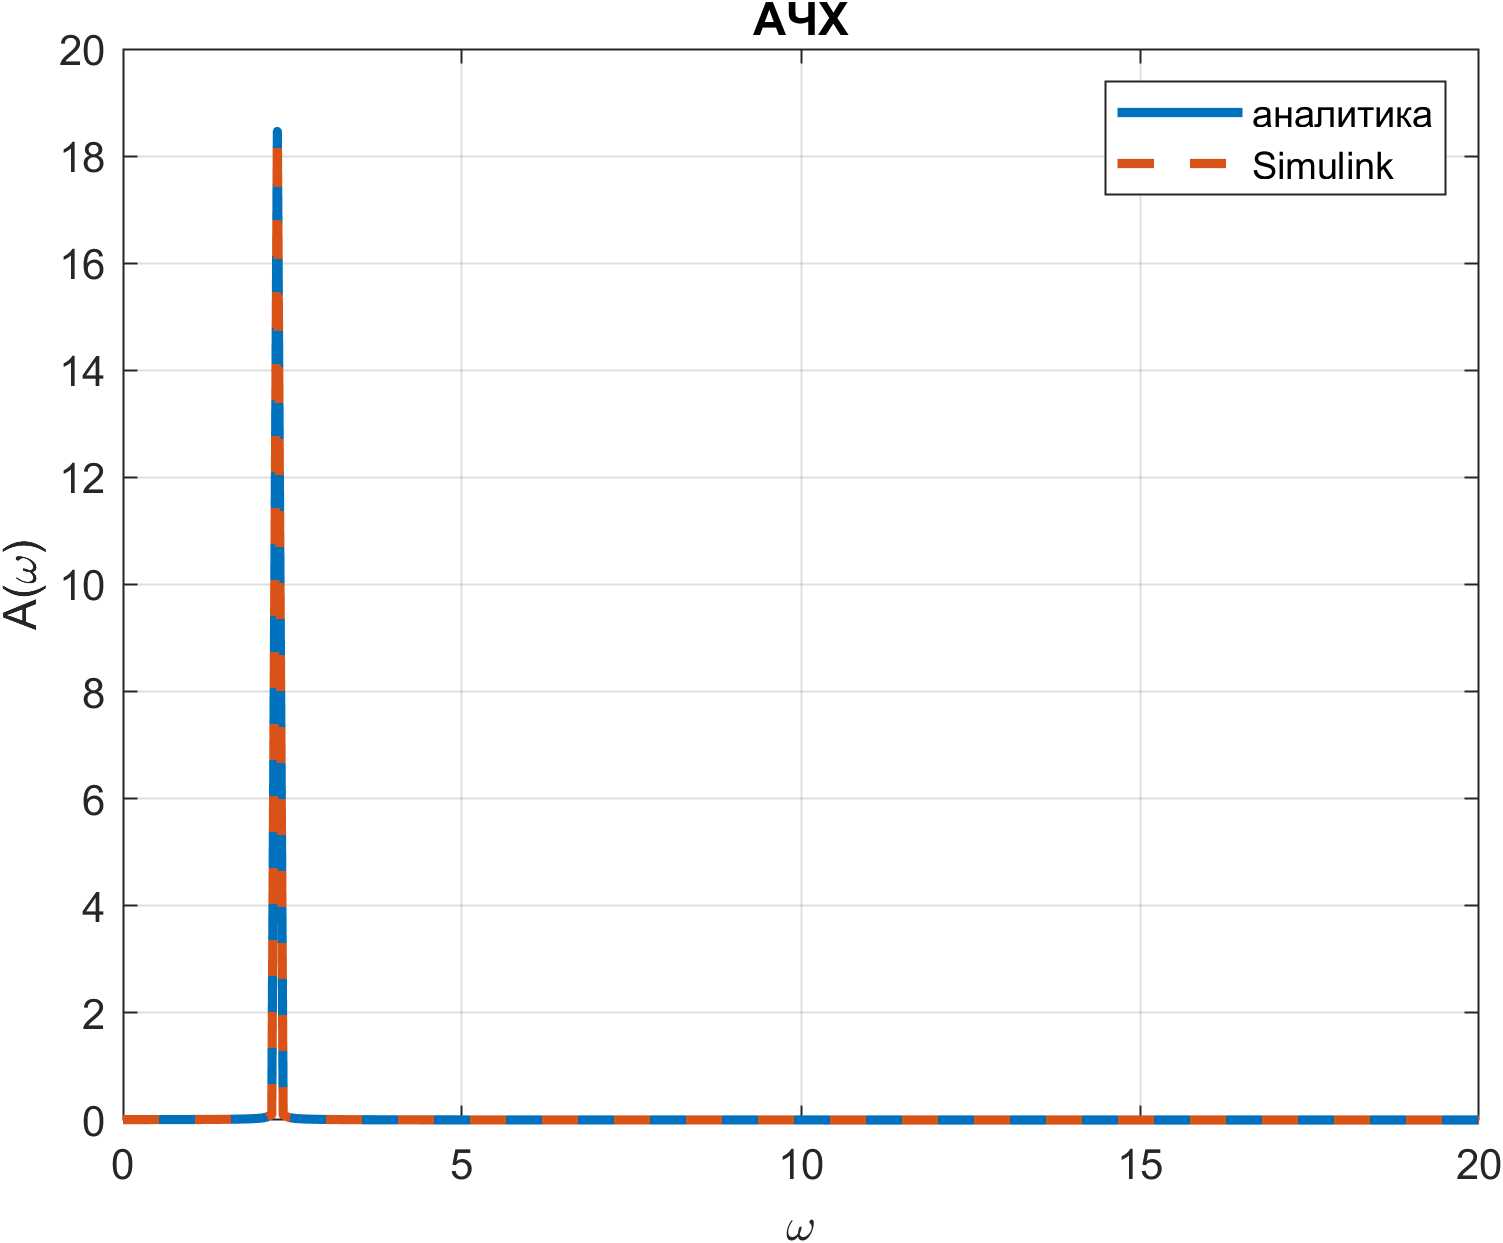
\includegraphics[width=0.8\textwidth]{images/ACH4.png}
    \caption{АЧХ системы}
    \label{fig:2}
\end{figure}

\begin{figure}[H]
    \centering
    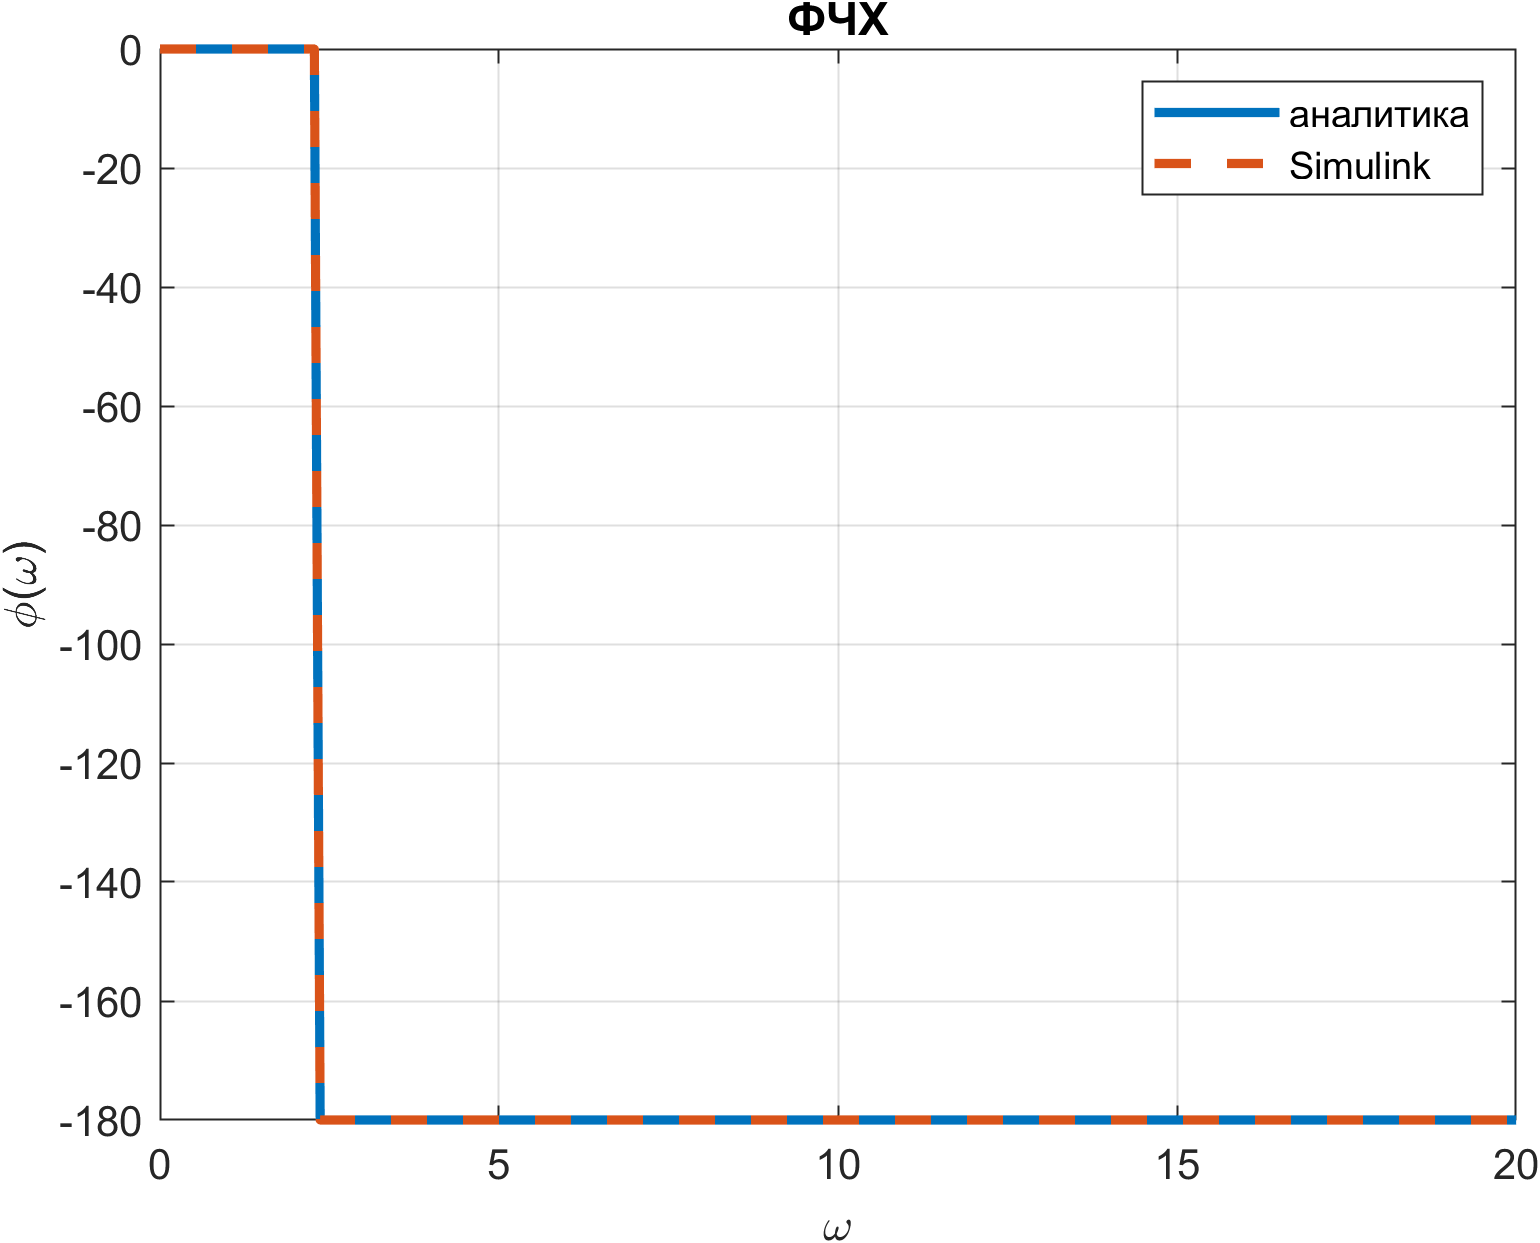
\includegraphics[width=0.8\textwidth]{images/FCH4.png}
    \caption{ФЧХ системы}
    \label{fig:2}
\end{figure}

\begin{figure}[H]
    \centering
    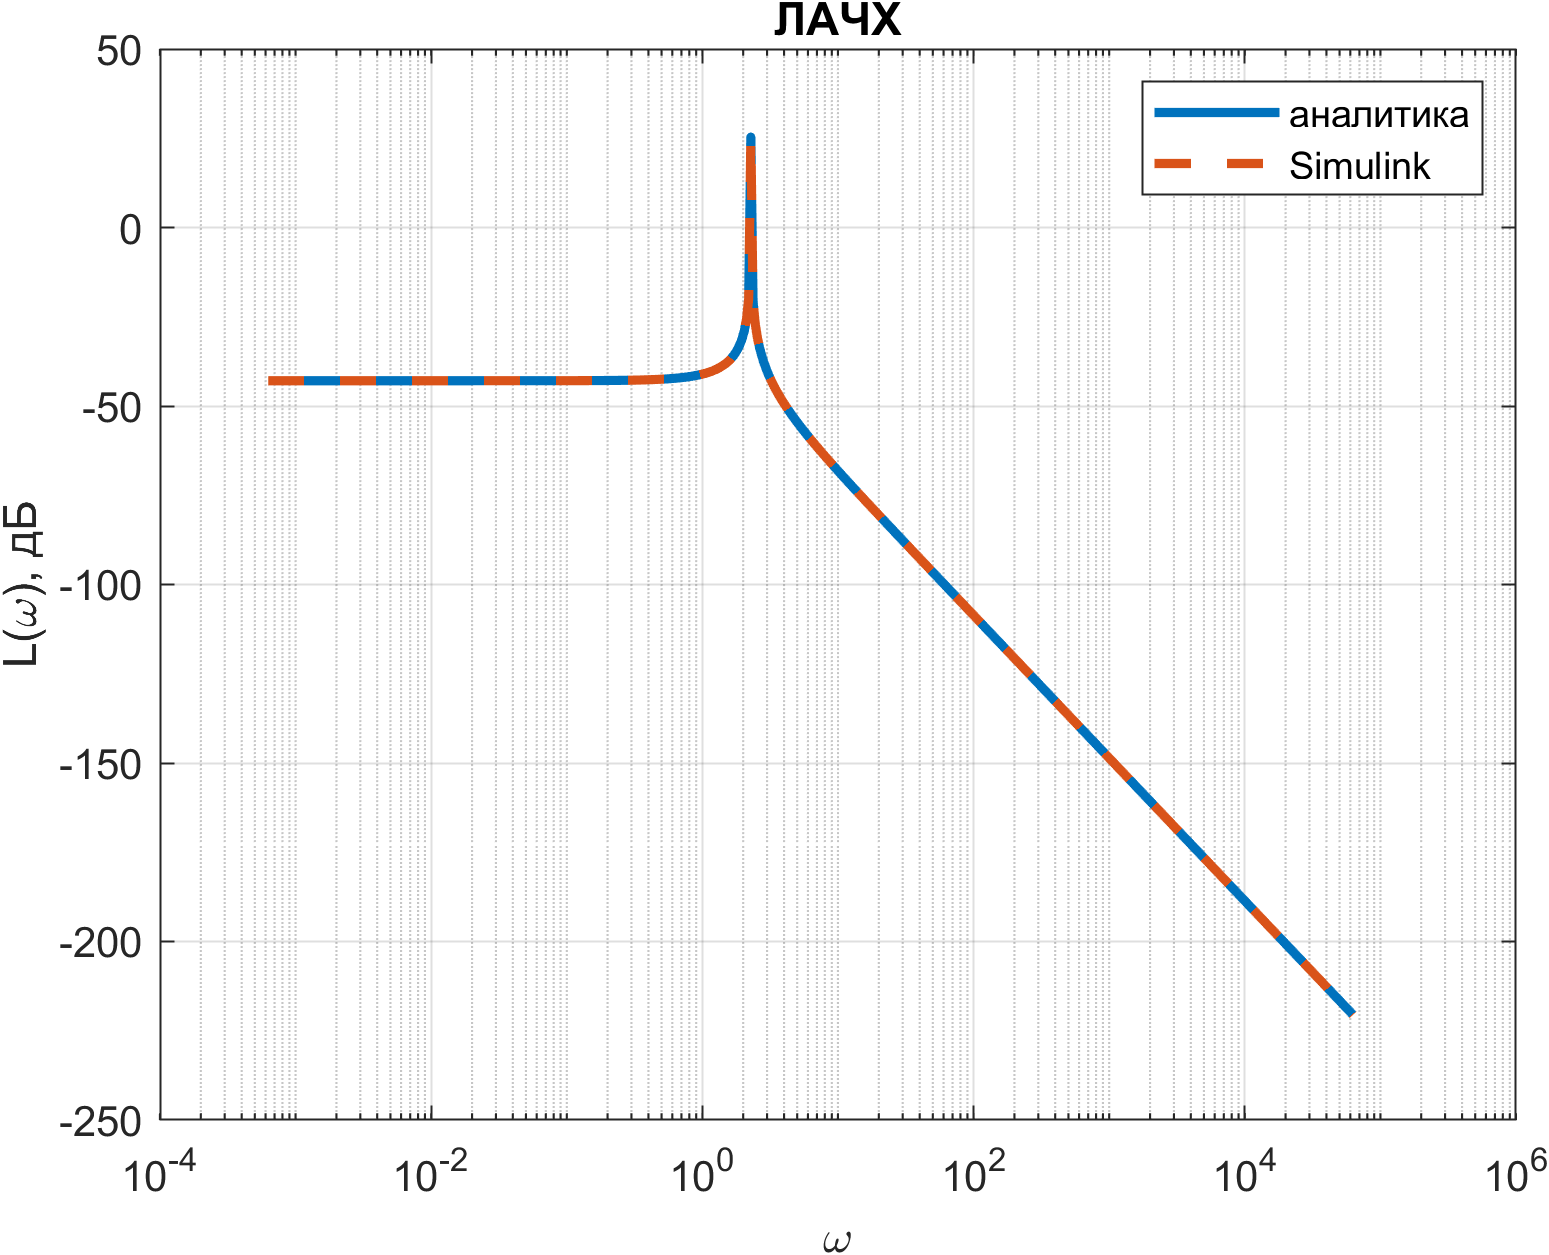
\includegraphics[width=0.8\textwidth]{images/LACH4.png}
    \caption{ЛАЧХ системы}
    \label{fig:2}
\end{figure}

\begin{figure}[H]
    \centering
    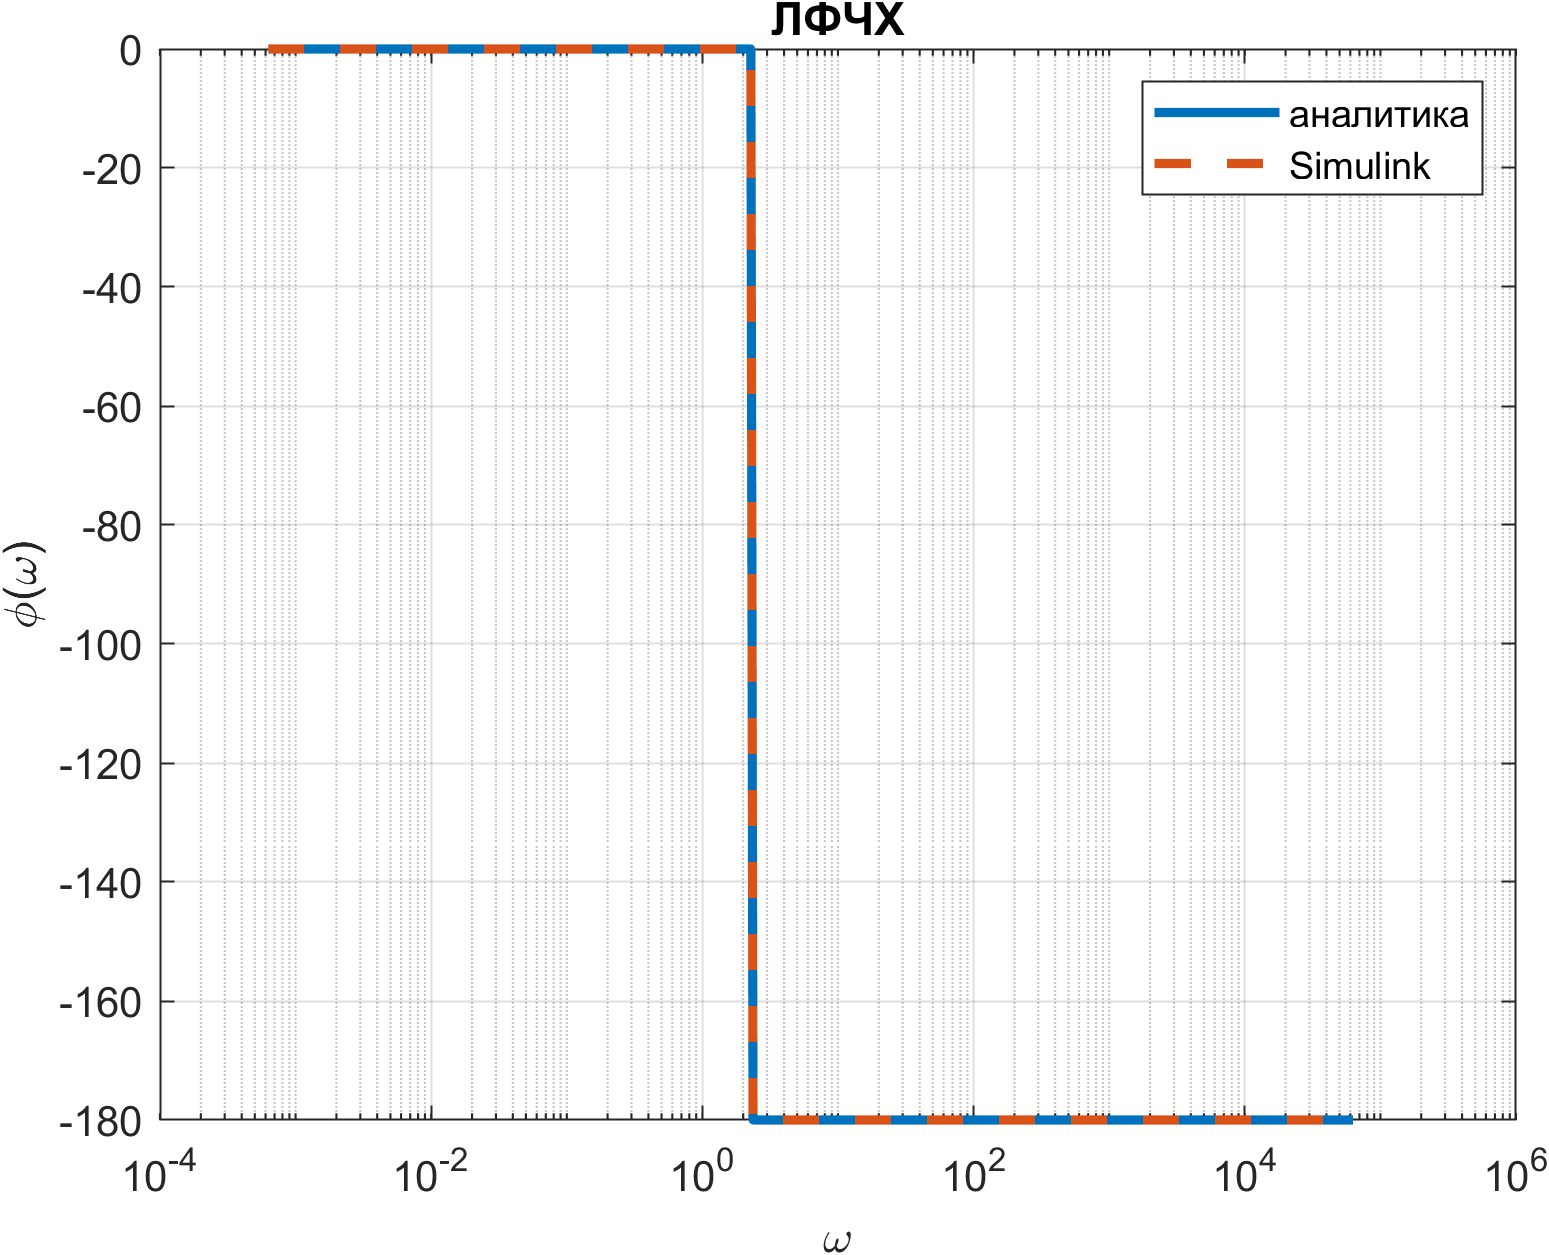
\includegraphics[width=0.8\textwidth]{images/LFCH4.png}
    \caption{ЛФЧХ системы}
    \label{fig:2}
\end{figure}  

\newpage
\section{Операционный усилитель}
\begin{figure}[H]
    \centering
    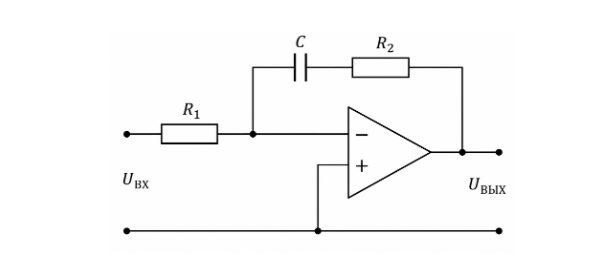
\includegraphics[width=0.8\textwidth]{images/schem2.png}
    \caption{Схема включения операционного усилителя}
    \label{fig:2}
\end{figure} 
Для данной схемы включения операционного усилителя можно записать передаточную функцию в виде

Ток через резистор $R_1$:
\begin{equation}
    i(t) = \frac{U_{\text{вх}}(t)}{R_1}.
\end{equation}

Этот же ток протекает через последовательно соединённые конденсатор $C$ и резистор $R_2$ в цепи обратной связи. Так как левый конец цепочки находится под потенциалом земли, имеем
\begin{equation}
    -U_{\text{вых}}(t) = u_C(t) + R_2\, i(t),
    \qquad
    \frac{du_C}{dt} = \frac{i(t)}{C}.
\end{equation}

Продифференцируем первое уравнение:
\begin{equation}
    -\frac{dU_{\text{вых}}}{dt} = \frac{i(t)}{C} + R_2\,\frac{di}{dt}.
\end{equation}

Подставим $i(t) = U_{\text{вх}}(t)/R_1$:
\begin{equation}
    -\frac{dU_{\text{вых}}}{dt}
    = \frac{U_{\text{вх}}}{R_1 C} + \frac{R_2}{R_1}\,\frac{dU_{\text{вх}}}{dt}.
\end{equation}

\begin{equation}
    \frac{dU_{\text{вых}}}{dt}
    = -\frac{R_2}{R_1}\,\frac{dU_{\text{вх}}}{dt} - \frac{1}{R_1 C}\,U_{\text{вх}},
\end{equation}
\begin{equation}
    R_1 C\,\frac{dU_{\text{вых}}}{dt}
    = -R_2 C\,\frac{dU_{\text{вх}}}{dt} - U_{\text{вх}}.
\end{equation}

Применяя преобразование Лапласа при нулевых начальных условиях, получим передаточную функцию:
\begin{equation}
    W(s) = -\frac{R_2 C s + 1}{R_1 C s}.
\end{equation}

Таким образом, схема является изодромным звеном с инверсией знака(которая игнорируется по заданию):
\begin{equation}
    W(s) = K\,\frac{T s + 1}{T s},
    \qquad T = R_2 C,\qquad K = \frac{R_2}{R_1}
\end{equation}
Тогда выражения для переходной и весовой характеристик
\[
\omega (t) = K\delta (t) + \frac{K}{T}
\]
\[
h(t) = K(1 + \frac{t}{T})
\]
Получим частотные характеристики. Подставим $s = i\omega$:
\[
W(i\omega) = K\,\frac{iT\omega + 1}{iT\omega} = K\left(1 - \frac{i}{T\omega}\right)
\]
Вещественная часть равна $K$, мнимая равна $-\dfrac{K}{T\omega}$, поэтому
\[
A(\omega) = K\sqrt{1 + \frac{1}{T^2\omega^2}} = \frac{K\sqrt{1 + T^2\omega^2}}{T\omega}
\]
\[
\varphi(\omega) = -\operatorname{arctg}\frac{1}{T\omega} = \operatorname{arctg}(T\omega) - \frac{\pi}{2}
\]
\[
L(\omega) = 20\lg K + 10\lg\left(1 + T^2\omega^2\right) - 20\lg(T\omega)
\]

Теперь зададимся параметрами
\[
R_1 = 2253, \qquad R_2 = 12964, \qquad C = 379
\]
И промоделируем систему.


\begin{figure}[H]
    \centering
    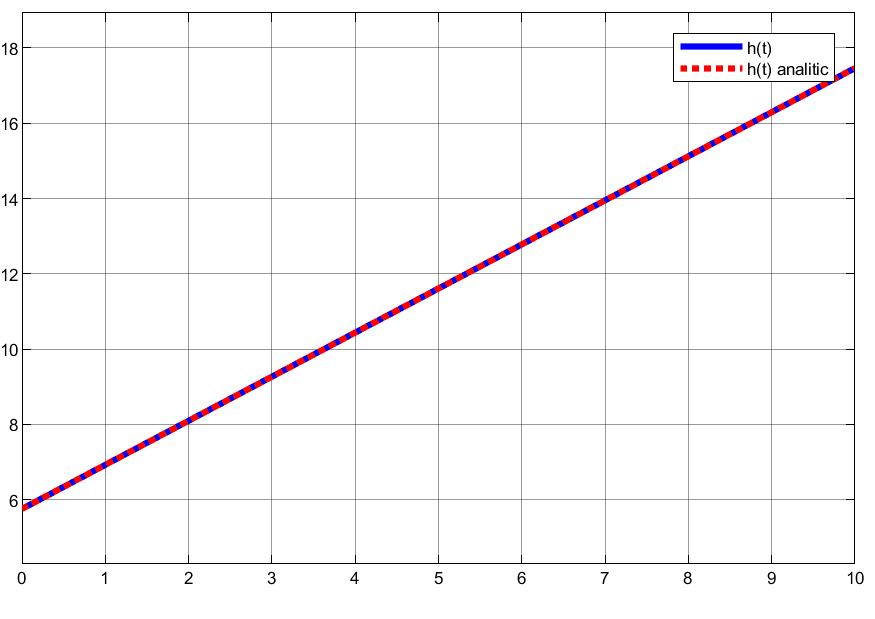
\includegraphics[width=0.8\textwidth]{images/h5.png}
    \caption{Переходная характеристика системы}
    \label{fig:2}
\end{figure}

\begin{figure}[H]
    \centering
    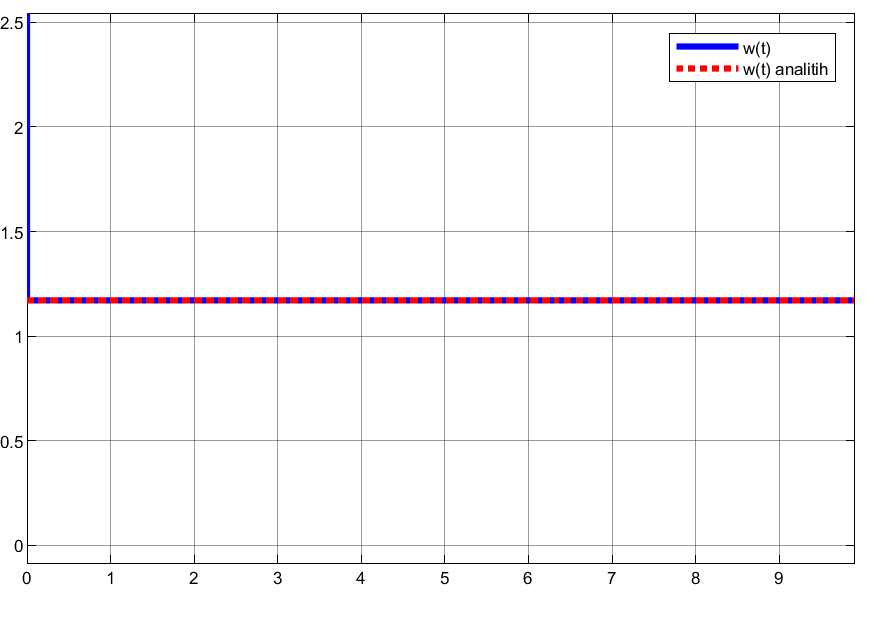
\includegraphics[width=0.8\textwidth]{images/w5.png}
    \caption{Весовая характеристика системы}
    \label{fig:2}
\end{figure}

\begin{figure}[H]
    \centering
    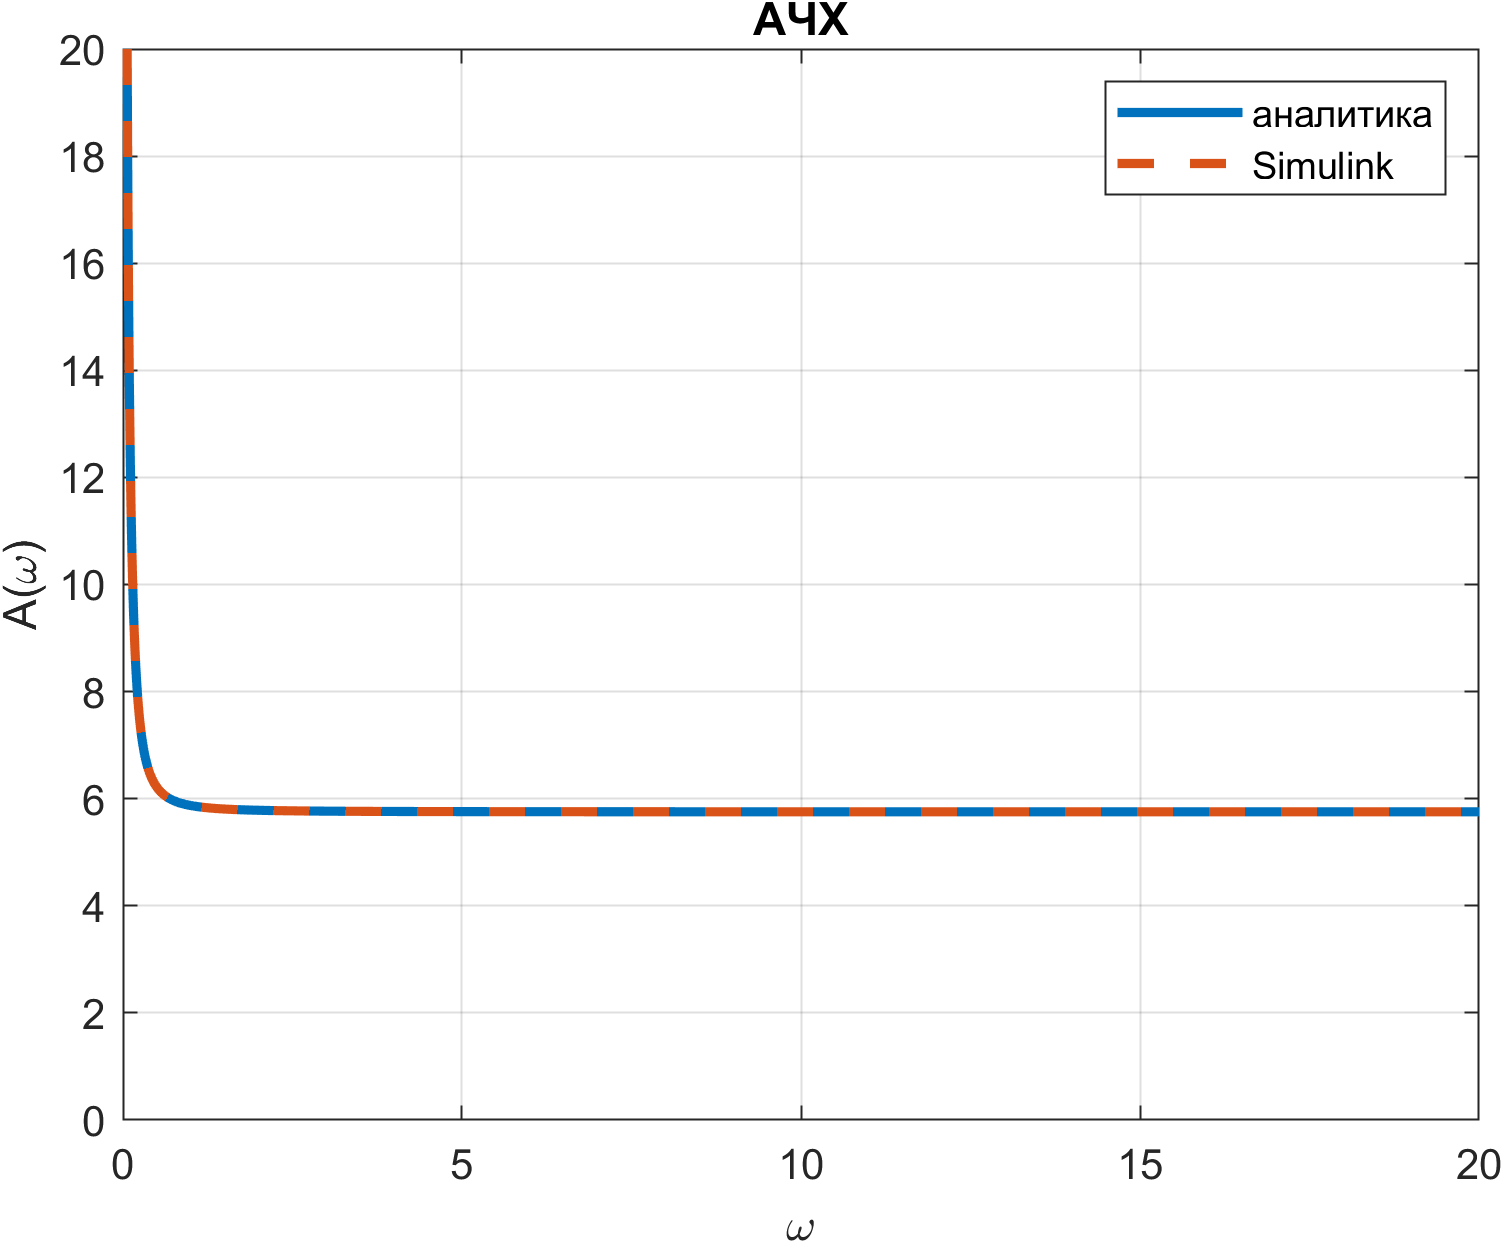
\includegraphics[width=0.8\textwidth]{images/ACH5.png}
    \caption{АЧХ системы}
    \label{fig:2}
\end{figure}

\begin{figure}[H]
    \centering
    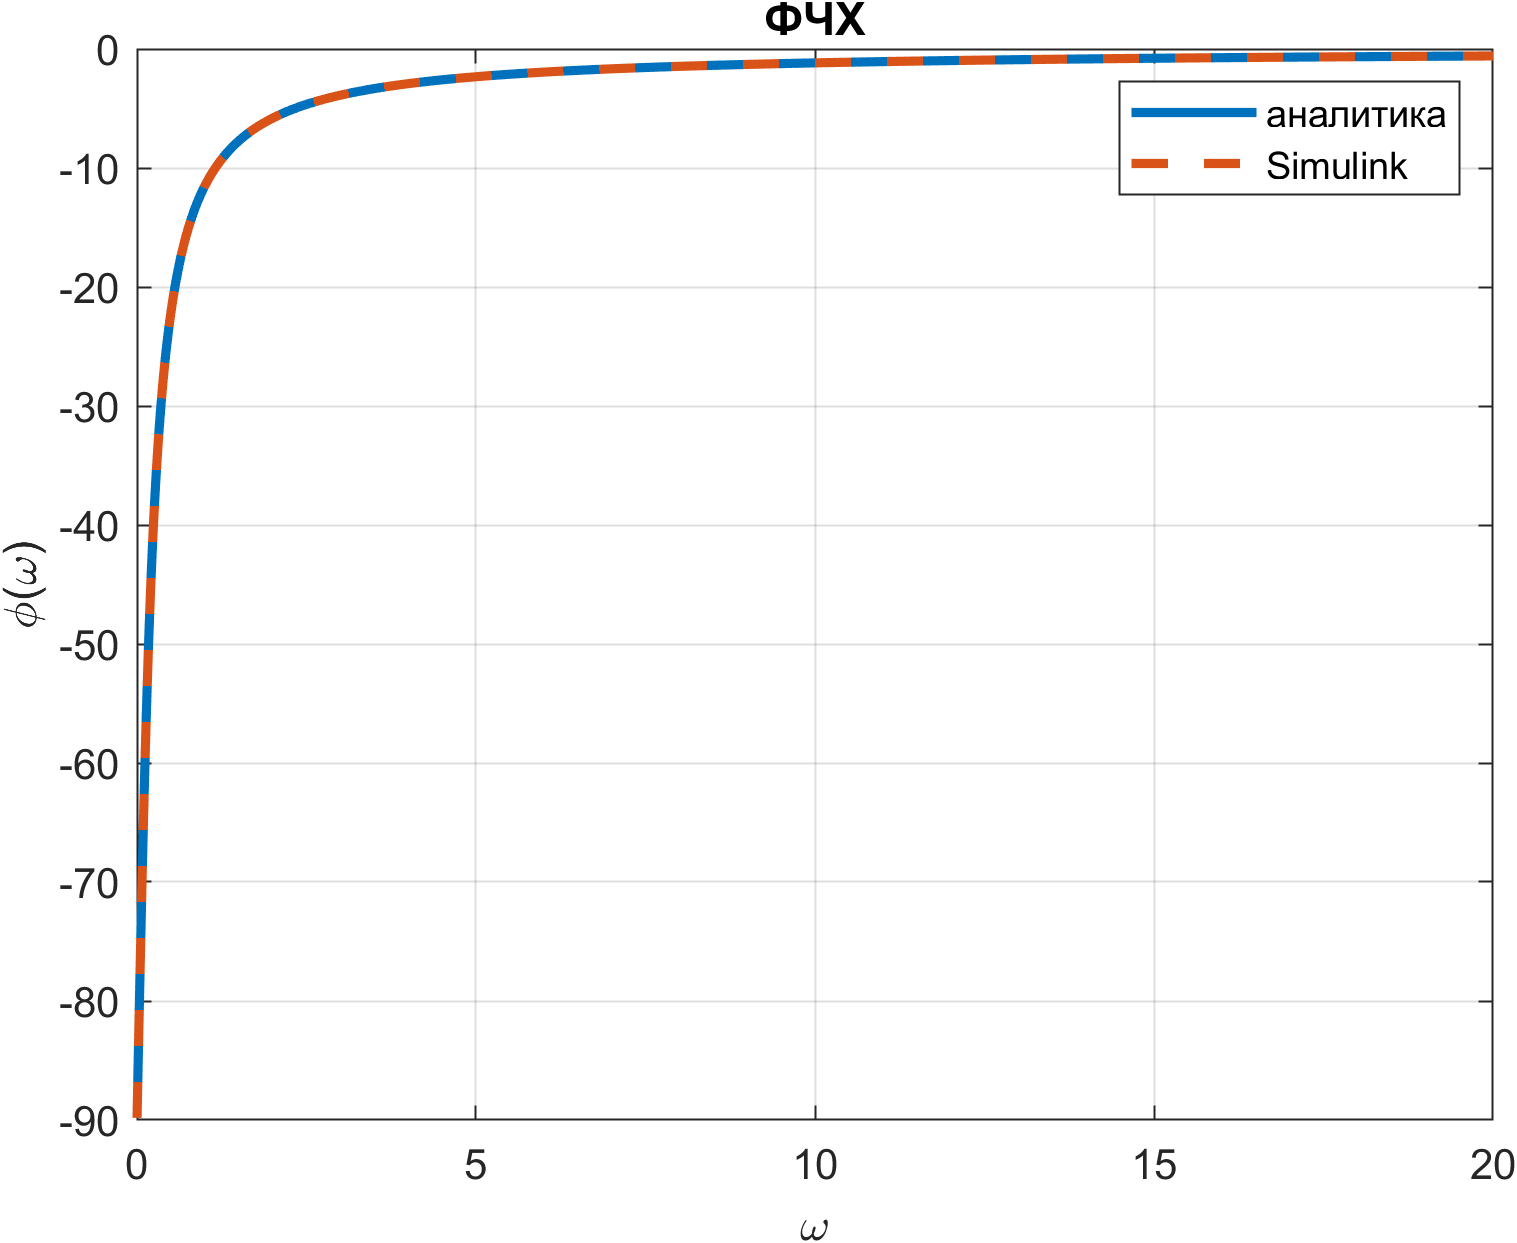
\includegraphics[width=0.8\textwidth]{images/FCH5.png}
    \caption{ФЧХ системы}
    \label{fig:2}
\end{figure}

\begin{figure}[H]
    \centering
    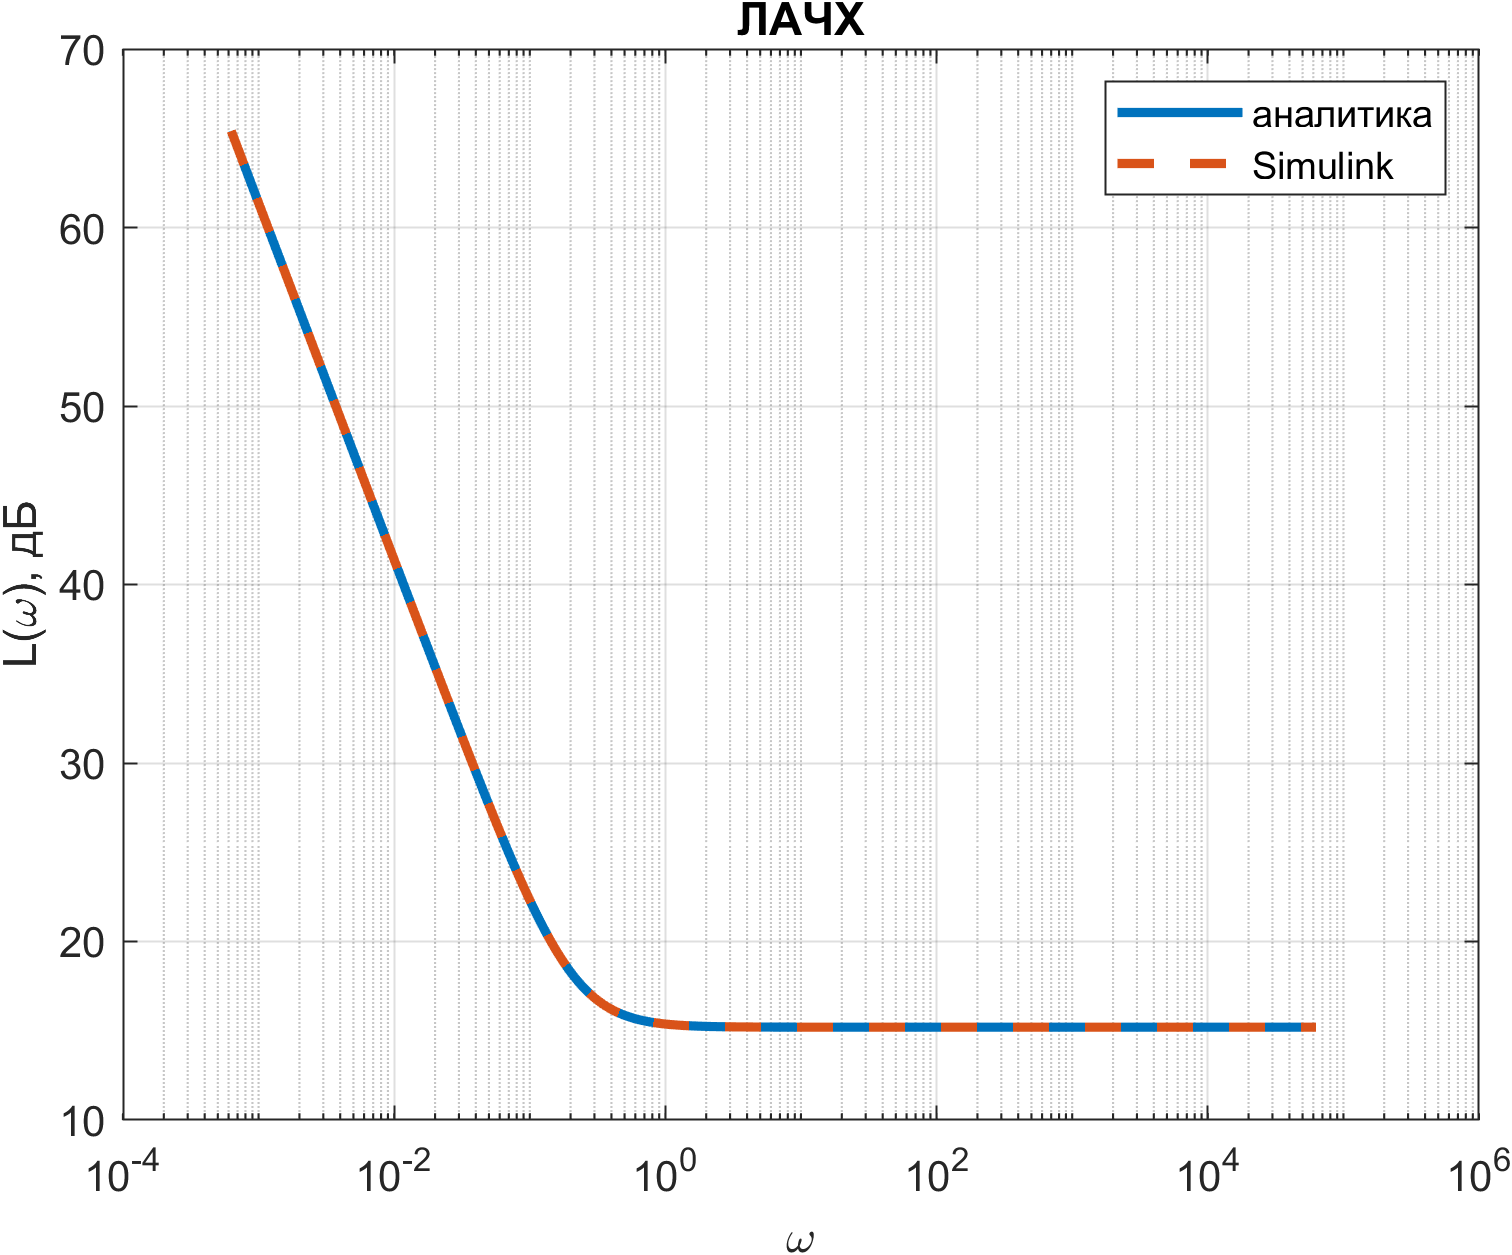
\includegraphics[width=0.8\textwidth]{images/LACH5.png}
    \caption{ЛАЧХ системы}
    \label{fig:2}
\end{figure}

\begin{figure}[H]
    \centering
    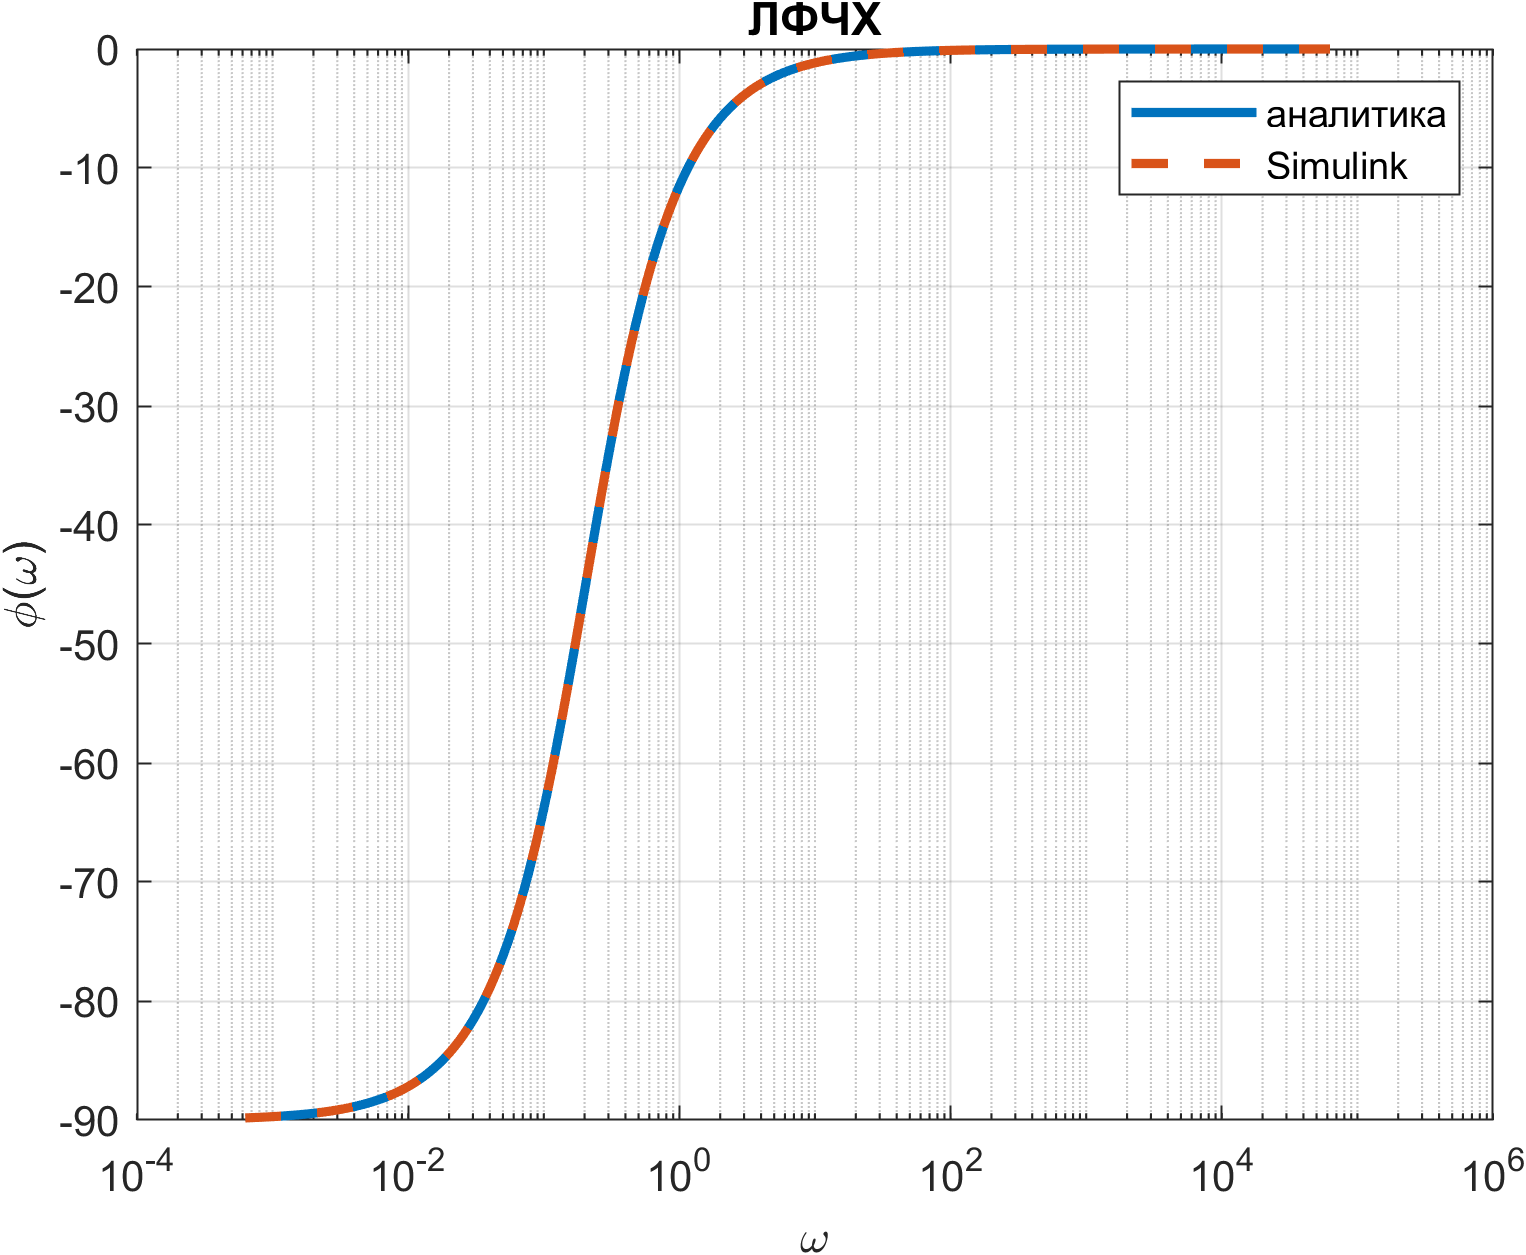
\includegraphics[width=0.8\textwidth]{images/LFCH5.png}
    \caption{ЛФЧХ системы}
    \label{fig:2}
\end{figure}  

\newpage
\section{Выводы}
В работе рассмотрены временные и частотные характеристики пяти типовых динамических звеньев, для каждого получены аналитические выражения передаточной функции, весовой и переходной функций, АЧХ, ФЧХ, ЛАЧХ и ЛФЧХ, и результаты сопоставлены с моделированием в Simulink.
\begin{itemize}
    \item Двигатель постоянного тока без учёта индуктивности является апериодическим звеном 1-го порядка с $K = 1/k_e \approx 3{,}10$ и $T \approx 0{,}124$ с. Его АЧХ монотонно убывает, фаза стремится к $-\pi/2$, наклон ЛАЧХ на высоких частотах равен $-20$ дБ/дек.
    \item При учёте индуктивности порядок системы повышается до второго. Для принятых параметров $T_m < 4T_e$, $\xi \approx 0{,}355 < 1$, поэтому звено колебательное: на АЧХ есть резонансный пик, фаза меняется от $0$ до $-\pi$, наклон ЛАЧХ на высоких частотах равен $-40$ дБ/дек, переходная характеристика колебательна. Учёт индуктивности заметно меняет динамику по сравнению с первой моделью.
    \item Конденсатор является идеальным дифференцирующим звеном. Его ЛАЧХ имеет наклон $+20$ дБ/дек, фаза постоянна и равна $+90^\circ$. Весовая и переходная функции содержат обобщённые функции ($\delta(t)$ и $\delta'(t)$), поэтому их можно показать лишь приближённо. Небольшое расхождение с Simulink на высоких частотах вызвано тем, что блок Derivative линеаризуется как $s/(cs + 1)$, а не как чистое $s$.
    \item Пружинный маятник без трения является консервативным звеном. Его полюса лежат на мнимой оси, на частоте $\omega_0 = \sqrt{k/M} \approx 2{,}28$ рад/с АЧХ обращается в бесконечность, фаза скачком меняется на $-\pi$. Затухание отсутствует, поэтому переходная характеристика представляет собой незатухающие колебания. Значения фазы $+180^\circ$ и $-180^\circ$ эквивалентны, различие связано только с выбором представления угла.
    \item Схема на операционном усилителе реализует изодромное звено $K(Ts + 1)/(Ts)$ с $K = R_2/R_1 \approx 5{,}75$ и $T = R_2C \approx 4{,}91$ с. На низких частотах оно ведёт себя как интегратор (наклон $-20$ дБ/дек, фаза $-90^\circ$), на высоких, как пропорциональное звено (уровень $20\lg K \approx 15{,}2$ дБ, фаза $0^\circ$). Знак минус, присущий схеме, при анализе амплитудных характеристик не учитывался.
\end{itemize}
Аналитические частотные характеристики в Simulink-моделировании согласуются с аналитическими результатами.

\newpage
\section{Код, для сравнения аналитических и симуляционных данных}
\begin{lstlisting}
    dir = 'C:\Users\Professional\Here i live\Uni\LSAC\lab4\Paper\images';
ke = 0.3222; km = 0.3222;
J = 0.0028; R = 4.6013; L = 1.1319;
%K  = 379e-6;
k = 140;
M = 27;
Tm = (J*R)/(km*ke);
Te = L/R;
R1 = 2253;
R2 = 12964;
C = 379e-6;
T = C*R2;
K = R2/R1;
%K = 1/k;
%T = sqrt(M/k);
%T  = sqrt(Tm*Te);
xi = T/(2*Te);
sig_xi  = xi/T;
omega_d = sqrt(1 - xi^2)/T;
mdl = 'model';
load_system(mdl);
io(1) = linio([mdl '/Sine Wave'],    1, 'input');
io(2) = linio([mdl '/Transfer Fcn2'], 1, 'output');
%io(2) = linio([mdl '/Derivative'], 1, 'output');
sys_lin = linearize(mdl, io);
f = logspace(-4, 4, 500);
w = 2*pi*f;
[mag_s, ph_s] = bode(sys_lin, w);
mag_s = squeeze(mag_s);
ph_s  = squeeze(ph_s);

mag_a = K*sqrt(1 + 1./(T*w).^2);
ph_a  = (atan(T*w) - pi/2)*180/pi;)
L_a   = 20*log10(K) + 10*log10(1 + (T*w).^2) - 20*log10(T*w);

wrap = @(p) mod(p + 180, 360) - 180;
ph_s = wrap(ph_s);
disp([K T xi])
disp([mag_a(1) mag_s(1)])
disp(mag_s(1)/mag_a(1))
L_s = 20*log10(mag_s);
idx = 1:20:numel(w);
fig = figure('Name','АЧХ');
plot(w, mag_a, '-', 'LineWidth', 2.2); hold on
plot(w, mag_s, '--', 'LineWidth', 2.2);
grid on; xlim([0 20]); ylim([0 20])
xlabel('\omega'); ylabel('A(\omega)')
title('АЧХ'); legend('аналитика','Simulink')
exportgraphics(fig, fullfile(dir, 'ACH5.png'), 'Resolution', 300);
fig = figure('Name','ФЧХ');
plot(w, ph_a, '-', 'LineWidth', 2.2);hold on
plot(w, ph_s, '--', 'LineWidth', 2.2);
grid on; xlim([0 20])
xlabel('\omega'); ylabel( '\phi(\omega)');
title('ФЧХ'); legend('аналитика','Simulink')
exportgraphics(fig, fullfile(dir, 'FCH5.png'), 'Resolution', 300);
fig = figure('Name','ЛАЧХ');
semilogx(w, L_a, '-', 'LineWidth', 2.2); hold on
semilogx(w, L_s, '--', 'LineWidth', 2.2);
grid on;
xlabel('\omega'); ylabel('L(\omega), дБ')
title('ЛАЧХ'); legend('аналитика','Simulink')
exportgraphics(fig, fullfile(dir, 'LACH5.png'), 'Resolution', 300);
fig = figure('Name','ЛФЧХ');
semilogx(w, ph_a, '-', 'LineWidth', 2.2); hold on
semilogx(w, ph_s, '--', 'LineWidth', 2.2);
grid on;
xlabel('\omega'); ylabel('\phi(\omega)')
title('ЛФЧХ'); legend('аналитика','Simulink')
exportgraphics(fig, fullfile(dir, 'LFCH5.png'), 'Resolution', 300);
\end{lstlisting}

\end{document}